\documentclass[a4paper,12pt,twoside]{book}

\usepackage[tmargin=15mm,bmargin=20mm,lmargin=20mm,rmargin=20mm]{geometry} % Formato de página

\usepackage[output-decimal-marker={,}]{siunitx} % Unidades del SI
    \sisetup{per-mode = fraction, fraction-function=\sfrac}
    \DeclareSIUnit{\rpm}{rpm}
    \DeclareSIUnit{\atmosphere}{atm}

\usepackage[framemethod=TikZ]{mdframed} % Define \begin{mdframed}[style=MyFrame1]

    \mdfdefinestyle{definicion-o-propiedad}
    {linecolor=black!80!gray,
    outerlinewidth=0.5pt,
    roundcorner=0pt,
    innertopmargin=15pt,
    innerbottommargin=20pt,
    innerrightmargin=15pt,
    innerleftmargin=15pt,
    backgroundcolor=gray!30!white}

    \mdfdefinestyle{ejercicio-facil}
    {linecolor=yellow,
    outerlinewidth=1pt,
    outerlinecolor=yellow,
    roundcorner=10pt,
    innertopmargin=10pt,
    innerbottommargin=10pt,
    innerrightmargin=10pt,
    innerleftmargin=10pt}

    \mdfdefinestyle{ejercicio-intermedio}
    {linecolor=orange,
    outerlinewidth=1pt,
    outerlinecolor=orange,
    roundcorner=10pt,
    innertopmargin=10pt,
    innerbottommargin=10pt,
    innerrightmargin=10pt,
    innerleftmargin=10pt}

    \mdfdefinestyle{ejercicio-dificil}
    {linecolor=red,
    outerlinewidth=1pt,
    outerlinecolor=red,
    roundcorner=10pt,
    innertopmargin=10pt,
    innerbottommargin=10pt,
    innerrightmargin=10pt,
    innerleftmargin=10pt}

    \mdfdefinestyle{ejercicio-conceptual}
    {linecolor=blue,
    outerlinewidth=1pt,
    outerlinecolor=blue,
    roundcorner=10pt,
    innertopmargin=10pt,
    innerbottommargin=10pt,
    innerrightmargin=10pt,
    innerleftmargin=10pt}

    \mdfdefinestyle{explicacion}
    {linecolor=gray!20!white,
    roundcorner=10pt,
    innertopmargin=10pt,
    innerbottommargin=10pt,
    innerrightmargin=10pt,
    innerleftmargin=10pt,
    backgroundcolor=gray!20!white}

\usepackage{graphicx}
    \graphicspath{{./images/}} % Define \graphicspath{{dir1}{dir2}} para incluir imágenes que estén en los directorios dir1 y dir2

\usepackage[spanish]{babel}  % Traducciones y abreviaturas
\usepackage{amssymb}  % Símbolos y tipografía matemáticos
\usepackage{amsmath}  % Formato y estructura matemáticos
\usepackage{esint} % Define \oiint para integrales cerradas y acomoda \iiint
\usepackage{hyperref}  % Referencias cruzadas
\usepackage{fancyhdr}  % Encabezado y pie
\usepackage{graphicx}  % Define \includegraphics
\usepackage{pdfpages} % Define \includepdf
\usepackage{multicol} % Entorno de formato en columnas
\usepackage{comment} % Comenta todo entre \begin{comment} \end{comment}
% COMANDOS DE FORMATO
\newcommand{\sub}[2]{{{#1}_\textsl{{#2}}}} % #1 subíndice #2 (Usado cuando #2 es $texto$)
\newcommand{\cusTi}[1]{\noindent\textbf{#1}} % Título de definiciones, propiedades, ejemplos y ejercicios
\newcommand{\cusTe}[1]{\vspace{2mm}\\\text{\hspace{\the\parindent}}#1} % Descripción de definiciones, propiedades, ejemplos y ejercicios
\newcommand{\noTi}[1]{\vspace{1ex}#1} % Descripción de definiciones, propiedades, ejemplos y ejercicios que no tengan título
\newcommand{\concept}[1]{\vspace{1ex} \textsc{#1}} % Subtítulos sin jerarquía
\newcommand{\braces}[1]{{ \left\{ {#1} \right\} }} % #1 entre llaves
\newcommand{\sqb}[1]{{ \begin{bmatrix} #1 \end{bmatrix} }} % #1 entre corchetes
\newcommand{\bb}[1]{\left(#1\right)} % #1 entre paréntesis
\newcommand{\sfrac}[2]{#1/#2} % Fracciones #1/#2 para reemplazar el (muy lento) \usepackage{xfrac}
\newcommand{\bq}[1]{``#1''}

% COMANDOS PARA NOTACIÓN DE FUNCIONES
\newcommand{\barrow}[3]{\begin{bmatrix} \left. #1 \right|_{#2}^{#3} \end{bmatrix}} % Regla de Barrow de #1 para los extremos de integración #2 y #3
\newcommand{\fx}[2][f]{#1 \hspace{-0.5mm} \left( #2 \right)} % #1 en función de #2 con paréntesis
\newcommand{\media}[2]{\underset{#2}{\sub{#1}{med}}} % #1 media entre #2
\newcommand{\norm}[1]{{\left| {#1} \right|}} % Módulo de #1
\newcommand{\nnorm}[1]{{\left|\left| {#1} \right|\right|}} % Norma de #1
\newcommand{\conj}[1]{\overline{#1}} % Conjugado de #1
\newcommand{\ave}[1]{\bar{#1}} % Valor promedio de #1

% COMANDOS PARA NOTACIÓN DE ELEMENTOS Y OPERADORES
\newcommand{\versor}[1]{\hat{#1}} % Vector unitario #1
\newcommand{\fasor}[1]{\check{#1}} % Fasor #1
\newcommand{\iVer}{\versor{\imath}} % i versor
\newcommand{\jVer}{\versor{\jmath}} % j versor
\newcommand{\kVer}{\versor{k}} % k versor
\newcommand{\eVer}{\versor{\textbf{e}}} % Versor canónico
\newcommand{\setO}{\varnothing} % Conjunto vacío
\newcommand{\setN}{\mathbb{N}} % Conjunto de los números naturales
\newcommand{\setZ}{\mathbb{Z}} % Conjunto de los números enteros
\newcommand{\setR}{\mathbb{R}} % Conjunto de los números reales
\newcommand{\setI}{\mathbb{I}} % Conjunto de los números imaginarios
\newcommand{\setC}{\mathbb{C}} % Conjunto de los números complejos
\newcommand{\iu}{\mathrm{i}\mkern1mu} % Unidad imaginaria o número i
\newcommand{\dif}{\textsl{d}} % Diferencial
\newcommand{\tq}{\hspace{1ex} \big/ \hspace{1ex}} % tal que

% COMANDOS PARA NOTACIÓN DE CONSTANTES Y MAGNITUDES
\newcommand{\peso}{\textsl{p}} % Peso
\newcommand{\xyz}{\vec{r}\hspace{0.05cm}} % Trayectoria [x(t),y(t),z(t)]
\newcommand{\m}{\si{\metre}} % Unidad metro
\newcommand{\km}{\si{\kilo\metre}} % Unidad kilómetro
\newcommand{\cm}{\si{\centi\metre}} % Unidad centímetro
\newcommand{\s}{\si{\second}} % Unidad segundo
\newcommand{\h}{\si{\hour}} % Unidad hora
\newcommand{\mps}{\si{\metre\per\second}} % Unidad metro por segundo
\newcommand{\mpss}{\si{\metre\per\second\squared}} % Unidad metro por segundo cuadrado
\newcommand{\kmph}{\si{\kilo\metre\per\hour}} % Unidad kilómetro por hora
\newcommand{\rpm}{\si{\rpm}} % Unidad revoluciones por minuto
\newcommand{\N}{\si{\newton}} % Unidad Newton
\newcommand{\Npm}{\si{\newton\per\metre}} % Unidad Newton por metro
\newcommand{\kg}{\si{\kilo\gram}} % Unidad kilogramo
\newcommand{\gr}{\si{\gram}} % Unidad gramo
\newcommand{\grps}{\si{\gram\per\second}} % Unidad gramo por segundo
\newcommand{\kgf}{\mathrm{kgf}} % Unidad kilogramo fuerza
\newcommand{\ms}{\milli\second} % Unidad milisegundo
\newcommand{\W}{\si{\watt}} % Unidad watt
\newcommand{\kWh}{\si{\kilo\watt\hour}} % Unidad kilowatt por hora

% ENTORNOS DE NUMERACIÓN
\newtheorem{defn}{{Definición}}[chapter]
\newtheorem{prop}{{Propiedad}}[chapter]
\newtheorem{ejercicio}{{Ejercicio}}[chapter]


\begin{document}

\pagestyle{fancy}
\fancyhf{}
\chead{\scriptsize \nouppercase\rightmark}
\cfoot{\scriptsize \thepage}
\pagenumbering{gobble}
\renewcommand{\headrulewidth}{0pt}

\frontmatter

\begin{center}
    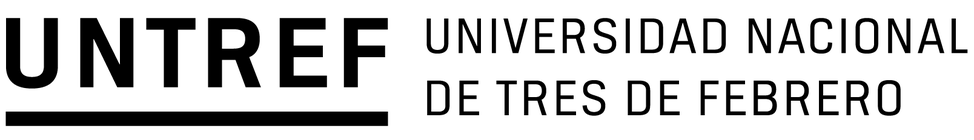
\includegraphics[width=0.5\linewidth]{untref.png}
    
    \vspace{10em}
    
    \begin{Large}
        Ingeniería de Sonido
    \end{Large}
    
    \vspace{2em}
    
    \begin{Huge}
        \textbf{Guía práctica de Física 1}
    \end{Huge}

    \vspace{2em}
    
    \textbf{Primera edición (v20230313)}
    
    \vspace{20em}

    \begin{small}
        \textbf{Docentes a cargo:}
    \end{small}

    \vspace{1ex}
    
    Escobar, Margarita R.
    \\
    mescobar@untref.edu.ar
    \\ \vspace{1em}
    Altamirano, Cecilia
    \\
    semproaltamirano@gmail.com
    \\ \vspace{1em}

    \begin{small}
        \textbf{Docentes adscriptos:}
    \end{small}

    \vspace{1ex}
    
    Malvicino, Maximiliano R.
    \\
    malvicino32646@estudiantes.untref.edu.ar
    \\ \vspace{1em}
    Veiga, Ignacio
    \\
    ignacioveigagiusti@mail.com

\end{center}

\clearpage
\noindent
\textbf{Introducción}

Los ejercicios están clasificados con diferentes colores de la siguiente manera.

\begin{mdframed}[style=ejercicio-conceptual]
    \cusTi{Ejercicio conceptual}
    \cusTe{Requieren un razonamiento que suele ser de carácter principalmente cualitativo. Ponen a prueba los conocimientos que son intuitivos contrastándolos con aquellos que no lo son.}
\end{mdframed}

\begin{mdframed}[style=ejercicio-facil]
    \cusTi{Ejercicio fácil}
    \cusTe{Generalmente usados como ejemplos para introducir los temas o incorporar métodos de resolución.}
\end{mdframed}

\begin{mdframed}[style=ejercicio-intermedio]
    \cusTi{Ejercicio intermedio}
    \cusTe{Diseñados para afianzar temas más complejos o profundizar un razonamiento analítico.}
\end{mdframed}

\begin{mdframed}[style=ejercicio-dificil]
    \cusTi{Ejercicio difícil}
    \cusTe{Abarcan varios temas, requieren conocer herramientas matemáticas determinadas y suelen ser usados como modelos de examen.}
\end{mdframed}

La versión más reciente de este texto puede ser descargada de:
\begin{center}
    \url{https://github.com/RosarioEs/guias_fisica_1}
    \\[1ex]
    \url{https://www.overleaf.com/read/ztdnzsbmyvxb}
\end{center}

Para más información, visitar el sitio web de la materia:
\begin{center}
    \url{https://sites.google.com/site/untrefisica1sonido}
\end{center}

\tableofcontents

\mainmatter
\pagenumbering{arabic}


\chapter{Cinemática}


\section{Sistemas y marcos de referencia}

\begin{mdframed}[style=explicacion]
    En física existen dos conceptos similares pero diferenciados para denominar al contexto de observación: marco de referencia (MR) y sistema de referencia (SR). 
    La ciencia es una actividad humana que consiste en la observación e interpretación de fenómenos de la realidad. Ese observador interpreta la realidad tomando en cuenta el contexto de los eventos y todas las variables que puedan intervenir en el movimiento o cambio de ese fenómeno a la luz de su conciencia, en un contexto determinado históricamente.
\end{mdframed}

\begin{mdframed}[style=ejercicio-conceptual]
    \begin{ejercicio}
    \end{ejercicio}
    \cusTi{Marcos y sistemas de referencia}
    \cusTe{(a) Clasificá las afirmaciones a continuación y decidí si refiere a un MR o a un SR o a ambos. Ubicalas en la tabla abajo.}
    
    \begin{enumerate}
        \item El lugar físico en donde se analizan los fenómenos, en particular, el movimiento.
        
        \item Cada punto de él representa una posición.
        
        \item Puede ser fijo o móvil respecto de otra cosa.
        
        \item Su movimiento o no es relativo sólo puede definirse en relación a otro.
        
        \item Se halla fijo respecto del observador dentro de él.
        
        \item Contienen información sobre las características del espacio en el que ocurre el movimiento: si es cilíndrico, esférico plano, o euclídeo.
        
        \item Pueden ser un tren, un departamento, un avión, un laboratorio, una plaza o un asiento en una montaña rusa.
        
        \item El conocimiento científico es el análisis y la interpretación de aquello que se mide en él.
        
        \item Un conjunto de coordenadas que representan el espacio.
        
        \item El espacio representado a través de un conjunto de coordenadas.
    \end{enumerate}

    \begin{center}
        \begin{tabular}{|c|c|}
            \hline
            SR & MR
            \\
            \hline
            &\\
            &\\
            &\\
            &\\
            &\\
            \hline
        \end{tabular}
    \end{center}

    (b) Ahora que ya ordenaste las definiciones. ¿Podés decir con tus palabras cuál es la diferencia entre un sistema de referencia y un marco de referencia?

    \vspace{1em}
    \emph{Sistema de referencia:}
    \vspace{4em}
    
    \emph{Marco de referencia:}
    \vspace{4em}
\end{mdframed}

\begin{mdframed}[style=ejercicio-conceptual]
    \begin{ejercicio}
    \end{ejercicio}
    \cusTi{Vectores posición, desplazamiento, velocidad y aceleración}
    \cusTe{    
    Un insecto pasa caminando por el punto
    $\vec{K} = 2 \, \si{\centi\metre} \, \iVer + 8 \, \si{\centi\metre} \, \jVer$.
    Tres segundos más tarde pasa por el punto
    $\vec{L} = 11 \, \si{\centi\metre} \, \iVer - 4 \, \si{\centi\metre} \, \jVer$.}

    \begin{enumerate}
        \item \concept{Vector posición}

        \begin{enumerate}
            \item Marcá en una hoja los dos puntos.
        
            \item Dibujale un marco de referencia posible.
            
            \item Completar:
            
            ``El punto ........ del sistema de referencia indica la ubicación del .....................''
            
            \item Indicá en el dibujo un sistema de referencia y dibujá el vector posición del insecto en cada uno de los puntos.
        
            \item En el sistema de referencia anterior, dibujá una posible trayectoria para el insecto.
            
            \item ¿Cuántas trayectorias posibles existen?
            
            \item Completar:
            
            ``La trayectoria es la curva que representa .......................................................''
        \end{enumerate}

        \item \concept{Vector desplazamiento}

        \begin{enumerate}
            \item Dibujar el vector desplazamiento del insecto en el esquema del ejercicio anterior con un color diferente al del vector posición.

            \item Marcar las opciones correctas. El vector desplazamiento del insecto anterior se expresa como:

            \begin{enumerate}
                \item $\vec{K} - \vec{L} = - 9 \, \si{\centi\metre} \, \iVer + 12 \, \si{\centi\metre} \, \jVer$

                \item $\vec{L} - \vec{K} = 9 \, \si{\centi\metre} \, \iVer - 12 \, \si{\centi\metre} \, \jVer$

                \item $\Delta \vec{r} = 9 \, \si{\centi\metre} \, \iVer - 12 \, \si{\centi\metre} \, \jVer$

                \item $\Delta \vec{r} = 9 \, \si{\centi\metre} \, \iVer + 4 \, \si{\centi\metre} \, \jVer$

                \item $\Delta \vec{r} = (9,-12,0)$

                \item $\Delta \vec{r} = (-9,12)$

                \item $\Delta\vec{r} = (9,-12)$
            \end{enumerate}
        \end{enumerate}
            
        \item \concept{Velocidad media e instantánea: determinar verdadero o falso o elegir la opción correcta según corresponda.}

        \begin{enumerate}
            \item La velocidad media/instantánea es la pendiente de la recta tangente a la trayectoria en un punto.

            \item La velocidad media/instantánea es la pendiente de la recta tangente a la posición en función del tiempo.

            \item La velocidad media es igual al cociente entre el vector desplazamiento y el tiempo transcurrido.

            \item La dirección y sentido de la velocidad media coincide con la dirección y sentido del vector desplazamiento.

            \item No se puede conocer la velocidad media del insecto del ejercicio anterior.

            \item Los vectores de velocidad se pueden dibujar en un espacio cartesiano que representa el espacio.

            \item Si la velocidad media del insecto es nula, significa que no se movió.

            \item Si la velocidad instantánea del insecto es nula, significa que el insecto no se mueve.

            \item No se puede conocer la velocidad media del insecto del ejercicio anterior.
            
            \item La velocidad media del insecto anterior es
            $\vec{v_m} = -3 \, \si{\centi\metre\per\second} \, \iVer + 4 \, \si{\centi\metre\per\second} \, \jVer$

            \item La velocidad media del insecto anterior es $5 \, \si{\metre\per\second}$

            \item La única manera de conocer la velocidad instantánea del insecto es derivando la posición en función del tiempo. 
        \end{enumerate}

        \item \concept{Aceleración media e instantánea: determinar verdadero o falso según corresponda.}
        
        \begin{enumerate}
            \item La aceleración es un vector que representa el cambio de la velocidad.

            \item Un cuerpo puede acelerarse sin la acción de otro cuerpo.

            \item La aceleración media coincide con la aceleración instantánea.
            
            \item La aceleración  es un vector paralelo a la velocidad.

            \item Si la aceleración media de un insecto es cero, significa que el insecto no se trasladó.

            \item La aceleración instantánea es la derivada de la velocidad instantánea.

            \item La aceleración media es el cociente entre la velocidad media entre dos puntos y el tiempo transcurrido en llegar de un punto al otro.

            \item Para conocer la aceleración, es necesario conocer antes la función velocidad.
        \end{enumerate}
    \end{enumerate}
\end{mdframed}

\begin{mdframed}[style=ejercicio-conceptual]
    \begin{ejercicio}
    \end{ejercicio}
    \noTi{La población $A$ de nuestra provincia de Buenos Aires está situada $160\,\km$ al este y $120\,\km$ al norte, con respecto a la ciudad $M$.}
    La población $B$ se sitúa $90\,\km$ al este y $120\,\km$ al sur, también con respecto a $M$.
    \begin{enumerate}
        \item Determiná el vector posición de las tres localidades.
        \item Una avioneta sale de $A$ a las $7\,\h$, y llega a $B$ a las $9\,\h$. Escribí su vector desplazamiento.
        \item En un esquema del lugar, dibujá dos trayectorias posibles diferentes, para cumplir el mismo viaje. ¿Cuántas hay?
        \item Encontrá el vector velocidad media de la avioneta en su viaje de $A$ hasta $B$, y calculá su módulo.
        \item A las $9:30\,\h$ la avioneta despega de $B$, y aterriza en $M$ a las $11\,\h$. Carga mercaderías y combustible y parte a las $15\,\h$, para llegar a la población $A$ a las $16:40\,\h$. Encontrá el vector velocidad media de la avioneta en cada uno de los intervalos indicados, y también para todo el viaje (desde las $7\,\h$ hasta las $16:40\,\h$).
        \item Escribir la dirección de los vectores velocidad media calculados en el ítem anterior.
    \end{enumerate}
\end{mdframed}


\section{Movimiento rectilíneo}


\subsection{Movimiento rectilíneo uniforme}

\begin{mdframed}[style=ejercicio-facil]
    \begin{ejercicio}
    \end{ejercicio}
    \noTi{Un automóvil se desplaza con velocidad constante por una sección recta de la Ruta Provincial número 4, yendo desde la ciudad de Laboulaye a la estación Fray Cayetano Rodríguez.}
    \begin{enumerate}
        \item Dibuje un sistema de referencia apropiado.
        \item ¿Cuál es su velocidad media si recorre el trayecto de $15 \si{\kilo\metre}$ en 10 minutos?
        \item A 7 kilómetros de Laboulaye, pasa por un lago. ¿Cuánto tiempo le tomó llegar al mismo?
        \item ¿Cuál es su velocidad instantánea al momento de pasar por el lago?
    \end{enumerate}
\end{mdframed}

\begin{mdframed}[style=ejercicio-facil]
    \begin{ejercicio}
    \end{ejercicio}
    \noTi{Una cuadrilla de empleados del ferrocarril viaja en una zorra por una vía rectilínea.}
    En un instante dado, por la misma vía y a $180\,\m$ por detrás, ven venir un tren que viaja con una velocidad constante de $36\,\kmph$.
    \begin{enumerate}
        \item ¿A qué velocidad mínima y constante deberá moverse la zorra para poder llegar a un desvío, que en ese instante está $120\,\m$ más adelante, para evitar el choque?
        \item Graficar velocidad y posición en función del tiempo, para ambos móviles
        \item Resolver ahora, considerando que se requieren 10 segundos para accionar el cambio de vía.
    \end{enumerate}
\end{mdframed}

\begin{mdframed}[style=ejercicio-facil]
    \begin{ejercicio}
    \end{ejercicio}
    \noTi{Un cuerpo, que en el instante $t = 0\,\s$ se encuentra en un punto $A$, viaja en línea recta con velocidad constante de módulo desconocido $v$.}
    Cuando transcurre un tiempo $T$ el móvil pasa por un punto $B$ que está a distancia $D$ de $A$.
    \begin{enumerate}
        \item Hallá $v$.
        \item Escribí dos expresiones para la posición del cuerpo en función del tiempo, una considerando un sistema de coordenadas con origen en $A$ y otra considerando un sistema de coordenadas con origen en $B$.
        \item Graficá las funciones definidas para el ítem anterior.
    \end{enumerate}
\end{mdframed}

\begin{mdframed}[style=ejercicio-facil]
    \begin{ejercicio}
    \end{ejercicio}
    \noTi{En cada uno de los gráficos se encuentra representado el movimiento de dos móviles.}
    \begin{center}
        \def\svgwidth{0.6\linewidth}
        \input{./images/ch1-mru-1.pdf_tex}
    \end{center}
    \begin{enumerate}
        \item Escribir las ecuaciones horarias correspondientes a los cinco primeros gráficos. Dar en cada caso las condiciones iniciales y, si corresponde, determinar cuándo se produce el encuentro.
        \item ¿Se pueden escribir las ecuaciones de posición en función del tiempo para ambos móviles en el sexto gráfico? ¿Se necesita algún dato adicional? ¿Se puede saber dónde se encuentran?
    \end{enumerate}
\end{mdframed}

\begin{mdframed}[style=ejercicio-intermedio]
    \begin{ejercicio}
    \end{ejercicio}
    \noTi{Un móvil, situado a una cierta distancia de otro, sale al encuentro de éste con velocidad uniforme.}
    Un instante después, el segundo móvil arranca con velocidad también constante.
    \begin{enumerate}
        \item Establecé un sistema de referencia.
        \item ¿Se van a encontrar los móviles?
        \item ¿Qué condiciones se tienen que cumplir para que se encuentren? Determinar las hipótesis necesarias y escribir esta condición matemáticamente.
        \item Suponiendo que en algún momento alguno de los dos autos tiene que doblar en una esquina, dibujá los vectores velocidad y aceleración en este caso.
    \end{enumerate}
\end{mdframed}

\begin{mdframed}[style=ejercicio-intermedio]
    \begin{ejercicio}
    \end{ejercicio}
    \noTi{Dos automóviles desean encontrarse en una ciudad que se encuentra entre sus posiciones actuales. Los dos viajarán por la misma ruta hacia la ciudad, la cual se encuentra en el kilómetro 45 de la ruta. Uno de los automóviles se encuentra en el kilómetro 10, y el otro en el kilómetro 60.}
    \begin{enumerate}
        \item Dibuje un sistema de referencia apropiado.
        \item ¿Cuánto les tomará llegar a destino si ambos conducen con una velocidad constante de $80\,  \kmph$? ¿Alguno llegará primero?
        \item ¿Cuál debería ser la velocidad del segundo automóvil para que lleguen a destino al mismo tiempo, considerando que el primero mantiene su velocidad de $80\,\si{\kilo\metre\per\hour}$?
        \item Si es el segundo auto el que conduce a $80\,  \si{\kilo\metre\per\hour}$, ¿Cuál debería ser la velocidad del primero para que se encuentren en el mismo instante?
        \item Si la velocidad máxima permitida es de $110\,  \si{\kilo\metre\per\hour}$, hay algún caso de los mencionados anteriormente en el que puedan ser detenidos por exceso de velocidad?
    \end{enumerate}
\end{mdframed}

    
\subsection{Movimiento rectilíneo uniformemente variado}

\begin{mdframed}[style=explicacion]
    El movimiento rectilíneo uniformemente variado (MRUV) se caracteriza por una trayectoria en línea recta con aceleración constante y distinta de cero.Por esta razón, la velocidad en este movimiento cambia uniformemente dependiendo de la dirección de la aceleración.
    Para poder identificar un MRUV es necesario conocer los parámetros que lo caracterizan:

    \begin{itemize}
        \item Su trayectoria es una recta, lo que significa que es un movimiento en una dimensión.
        \item Su aceleración es distinta de cero
        \item Su velocidad varía en forma constante como consecuencia de esa  aceleración. 
    \end{itemize}

    En un MRUV la aceleración es constante, nunca va a cambiar, siempre es la misma.
    ¡Pero mucha atención!
    Lo que es constante es la aceleración, no la velocidad.
    A tener muy en cuenta:

    \begin{itemize}
        \item La gráfica de la posición en función del tiempo es una parábola.
        \item La gráfica de la velocidad en función del tiempo es una recta cuya pendiente es la aceleración.
        \item Los signos tanto de la velocidad como de la aceleración dependen del sistema de referencia tomado. Esto quiere decir que la velocidad y la aceleración pueden ser positivas o negativas, e incluso nula en el caso de la velocidad, y esto solo va a depender del sistema de referencia elegido.
        \item Para poder determinar si un móvil está acelerando o frenando basta con examinar los signos de la velocidad y la aceleración en un instante dado. Si los signos de ambas magnitudes son opuestos, el móvil está desacelerando.
    \end{itemize}

    Es muy importante escribir las ecuaciones de movimiento para poder ir registrando los datos que se tienen y los datos que faltan. Atención al establecer las condiciones iniciales y sobre todo, no olvidar el sistema de referencia.
\end{mdframed}

\begin{mdframed}[style=ejercicio-facil]
    \begin{ejercicio}
    \end{ejercicio}
    \noTi{Un cohete parte del reposo con aceleración constante y logra alcanzar en $30\,\si{\second}$ una velocidad de $588\,\si{\metre\per\second}$.}
    \begin{enumerate}
        \item Calcular la aceleración del cohete.
        \item ¿Qué espacio recorrió en esos 30 s?
    \end{enumerate}
\end{mdframed}

\begin{mdframed}[style=ejercicio-facil]
    \begin{ejercicio}
    \end{ejercicio}
    \noTi{Un motociclista parte del reposo y tarda $10\,\si{\second}$ en recorrer $20\,\si{\metre}$. ¿Qué tiempo necesitará para alcanzar $40\,\si{\kilo\metre\per\hour}$?}
\end{mdframed}

\begin{mdframed}[style=ejercicio-facil]
    \begin{ejercicio}
    \end{ejercicio}
    \noTi{Un móvil parte del reposo con una aceleración de $20\,\si{\metre\per\second\squared}$ constante.}
    \begin{enumerate}
        \item ¿Qué velocidad tendrá después de $15\,\si{\second}$?
        \item ¿Qué espacio recorrió en esos $15\,\si{\second}$?
    \end{enumerate}
\end{mdframed}

\begin{mdframed}[style=ejercicio-facil]
    \begin{ejercicio}
    \end{ejercicio}
    \noTi{Un móvil que se desplaza con velocidad constante aplica los frenos durante $25\,\si{\second}$ y recorre $400\,\si{\metre}$ hasta detenerse.}
    \begin{enumerate}
        \item ¿Qué velocidad tenía el móvil antes de aplicar los frenos?
        \item ¿Qué desaceleración produjeron los frenos?
    \end{enumerate}
\end{mdframed}

\begin{mdframed}[style=ejercicio-facil]
    \begin{ejercicio}
    \end{ejercicio}
    \noTi{Un automóvil cuya velocidad es $90\,\kmph$ pasa ante un puesto caminero.}
    En ese instante sale en su persecución un patrullero que parte del reposo y acelera uniformemente durante todo el recorrido.
    Sabiendo que el patrullero alcanza una velocidad de $90\,\kmph$ en $10\,\s$, hallar:
    \begin{enumerate}
        \item El tiempo que dura la persecución.
        \item La posición en que el patrullero alcanza el automóvil.
        \item La velocidad del patrullero en dicho punto.
        \item Graficar, para ambos móviles, la velocidad en función del tiempo y relacionar dicho gráfico con las respuestas a las preguntas anteriores.
    \end{enumerate}
\end{mdframed}

\begin{mdframed}[style=ejercicio-intermedio]
    \begin{ejercicio}
    \end{ejercicio}
    \noTi{Analizar el gráfico dado, que corresponde a un movimiento rectilíneo en varias etapas.}
    \begin{center}
        \def\svgwidth{0.5\linewidth}
        \input{./images/ch1-mruv-1.pdf_tex}
    \end{center}
    Suponiendo que en $t=0$ es $x=0$, se pide:
    \begin{enumerate}
        \item Trazar los gráficos de aceleración y de posición en función del tiempo, determinando los valores correspondientes a los tiempos indicados.
        \item Calcular la velocidad media del móvil, entre $0\,\si{\second}$ y $25\,\si{\second}$. Prestar mucha atención a la definición de la magnitud que se está pidiendo.
        \item Desde la mecánica newtoniana, ¿qué implica que un cuerpo esté acelerado?
    \end{enumerate}
\end{mdframed}

\begin{mdframed}[style=ejercicio-intermedio]
    \begin{ejercicio}
    \end{ejercicio}
    \noTi{Un automóvil viaja en línea recta desde $A$ hasta $C$, con velocidad constante, pasando por $B$. Se sabe que por $A$ pasa a las $12\,\si{\hour}$, por $B$ a las $13\,\si{\hour}$ y por $C$ a las $15\,\si{\hour}$. Se sabe que $\overline{AB} = 50\,\si{\kilo\metre}$ pero $\overline{BC}$ es desconocido.}
    \begin{enumerate}
        \item Elegir un origen de tiempo y un sistema de referencia.
        \item Elegir un instante $t_0$. ¿Cuánto vale $x_0$? Escribir la ecuación de movimiento.
        \item Elegir otro instante $t_0$ ¿Cuánto vale $x_0$?
        \item Escribir la ecuación de movimiento.
        \item Calcular la velocidad del auto y la distancia $\overline{BC}$.
    \end{enumerate}
\end{mdframed}

\begin{mdframed}[style=ejercicio-intermedio]
    \begin{ejercicio}
    \end{ejercicio}
    \noTi{Observar detenidamente los gráficos de posición ($x$) en función del tiempo ($t$) que están a continuación.}
    \begin{center}
        \def\svgwidth{0.8\linewidth}
        \input{./images/ch1-mruv-2.pdf_tex}
    \end{center}
    \begin{enumerate}
        \item
        Sin usar valores numéricos, determinar los signos de la posición, la aceleración y la velocidad en $t=0\,\si{\second}$. Para cada caso, graficar la velocidad y la aceleración en función del tiempo.
        \item
        Suponer para los gráficos superiores $\norm{x(t=0)}=1\,\si{\metre}$ y $\norm{v(t=0)}=2\,\si{\metre\per\second}$ a menos que sea nula. Para los gráficos inferiores suponer $\norm{x(t=0)}=3\,\si{\metre}$ y $\norm{v(t=0)}=4\,\si{\metre\per\second}$ a menos que sea nula y escribir explícitamente las ecuaciones de posición considerando en todos los casos que $\norm{a}=6\,\si{\metre\per\second\squared}$.
    \end{enumerate}
\end{mdframed}

\begin{mdframed}[style=ejercicio-intermedio]
    \begin{ejercicio}
    \end{ejercicio}
    \noTi{Un auto viaja por una ruta recta a $20\,\si{\metre\per\second}$ y un perro se cruza frente a éste $50\,\si{\metre}$ adelante.}
    \begin{enumerate}
        \item ¿Cómo deben ser los sentidos de los vectores aceleración y velocidad para que el auto frene?
        \item ¿Cuál es la desaceleración mínima que debe imprimirse al automóvil para no chocar al perro?
        \item ¿Cuál es la desaceleración mínima que debe imprimirse al automóvil para no chocar al perro, teniendo en cuenta que el tiempo de respuesta del chofer es $0.3\,\si{\second}$?
        \item Mostrar simultáneamente ambas situaciones en un gráfico de $x$ en función de $t$.
    \end{enumerate}
\end{mdframed}

\begin{mdframed}[style=ejercicio-intermedio]
    \begin{ejercicio}
    \end{ejercicio}
    \noTi{Un automovilista se da cuenta al sobrepasar a un motociclista que se trata de un amigo e instantáneamente aplica los frenos.
    Se desprecia el tiempo de reacción.
    El siguiente gráfico de $v(t)$ representa el comportamiento de cada vehículo, en el que se ha cronometrado la velocidad en el instante en que el auto sobrepasa la moto.}
    \begin{center}
        \def\svgwidth{0.5\linewidth}
        \input{./images/ch1-mruv-3.pdf_tex}
    \end{center}
    \begin{enumerate}
        \item ¿Qué vehículo va adelante $4\,\si{\second}$ después que el auto pasa la moto? ¿O van juntos? 
        \item ¿Cuándo y dónde vuelven a encontrarse?
        \item ¿Cuál es la velocidad del auto en ese momento?
        \item Graficar $x(t)$ para ambos móviles.
    \end{enumerate}
\end{mdframed}

\begin{mdframed}[style=ejercicio-dificil]
    \begin{ejercicio}
    \end{ejercicio}
    \noTi{El siguiente gráfico representa la velocidad en función del tiempo para un automóvil que se desplaza en línea recta.}
    \begin{center}
        \def\svgwidth{0.6\linewidth}
        \input{./images/ch1-mruv-5.pdf_tex}
    \end{center}
    Suponiendo que el automóvil parte en $t=0$ de $x=0$ se pide:
    \begin{enumerate}
        \item Definir las ecuaciones horarias del cuerpo.
        \item Realizar el gráfico que representa la posición del cuerpo en función del tiempo.
        \item Indicar el valor de la posición a los $12\,\s$.
    \end{enumerate}
\end{mdframed}

    
\subsubsection{Caída libre y tiro vertical}

\begin{mdframed}[style=explicacion]
    Ambos movimientos son casos particulares de MRUV, por lo tanto van a tener una aceleración constante: la de la gravedad. El vector $\Vec{g}$ siempre apunta hacia el centro de la Tierra, lo cual no quiere decir que tenga necesariamente signo positivo o negativo. El signo de $\Vec{g}$ al igual que el de cualquier vector, dependerá del sistema de referencia adoptado. Es muy importante escribir las ecuaciones horarias al principio del ejercicio, para poder ir registrando los datos que se tienen y los datos que faltan. Prestar especial atención al establecer las condiciones iniciales y sobre todo, no olvidar el sistema de referencia.
    La velocidad y la aceleración tendrán el mismo signo en una caída libre, y signo contrario en un tiro vertical, independientemente del sistema de referencia elegido, sin necesidad de cambiar el sistema de referencia para un caso u otro. Es decir, si se lanza un objeto verticalmente, no hace falta dividir el problema en dos tramos, pues si las ecuaciones están bien escritas, ellas mismas determinarán el signo de la velocidad. 
\end{mdframed}

\begin{mdframed}[style=ejercicio-facil]
    \begin{ejercicio}
    \end{ejercicio}
    \noTi{Un cuerpo cae libremente desde el reposo. Calcular:}
    \begin{enumerate}
        \item La distancia recorrida en $3\,\s$.
        \item La velocidad después de haber recorrido $100 \, \m$.
        \item El tiempo necesario para alcanzar una velocidad de $25 \, \mps$.
        \item El tiempo necesario para recorrer $300 \, \m$, desde que cae.
    \end{enumerate}
\end{mdframed}

\begin{mdframed}[style=ejercicio-facil]
    \begin{ejercicio}
    \end{ejercicio}
    \noTi{Horacio decide lanzar una manzana desde su balcón  hacia la cabeza de su compañero de trabajo que justo pasa por la vereda en ese instante.
    Si la manzana llega a la cabeza del compañero en 5 s:}
    \begin{enumerate}
        \item ¿En qué piso vive Horacio, si cada piso mide $3 \, \m$?
        \item ¿Con qué velocidad llega?
    \end{enumerate}
\end{mdframed}

\begin{mdframed}[style=ejercicio-intermedio]
    \begin{ejercicio}
    \end{ejercicio}
    \noTi{Con el propósito de pedir un deseo, el señor Amilcar Bonifacini deja caer una piedra en un pozo.
    Al cabo de 10 segundos oye el choque contra el fondo.
    El señor Amilcar sabe que la velocidad del sonido es de $330 \, \mps$ y utiliza este dato para conocer la profundidad del pozo.
    ¿Cuál es la profundidad del pozo de los deseos calculada por el señor Bonifacini?}
\end{mdframed}

\begin{mdframed}[style=ejercicio-facil]
    \begin{ejercicio}
    \end{ejercicio}
    \noTi{Una bala se dispara verticalmente hacia arriba, y adquiere una velocidad inicial de $200 \, \mps$.}
    Determinar si al cabo de $20 \, \s$, la bala está subiendo o está descendiendo, y a qué altura se encuentra la misma.
\end{mdframed}

\begin{mdframed}[style=ejercicio-facil]
    \begin{ejercicio}
    \end{ejercicio}
    \noTi{Raquel no tiene nada mejor que hacer que ponerle un velocímetro a un cascote que se encontró en la estación de Villa Bosch.}
    Decide tirar el cascote desde una altura solo conocida por ella y partiendo siempre desde el reposo.
    ¿Cuál será la lectura del velocímetro a los 4, 5, 8 y 100 segundos?
\end{mdframed}

\begin{mdframed}[style=ejercicio-facil]
    \begin{ejercicio}
    \end{ejercicio}
    \noTi{Un colectivo de la línea 180 choca a $60 \, \kmph$ contra el paredón de la cancha de Nueva Chicago.}
    Un hincha que observó el siniestro se preguntó lo siguiente: ¿Desde qué altura habría que dejar caer al colectivo para producir el mismo efecto?
\end{mdframed}

\begin{mdframed}[style=ejercicio-facil]
    \begin{ejercicio}
    \end{ejercicio}
    \noTi{Se lanza un objeto desde una cierta altura del suelo sobre la superficie de la Tierra.}
    Suponiendo que no hay rozamiento:
    \begin{enumerate}
        \item ¿Cuánto tarda en llegar al suelo?
        \item ¿Con qué velocidad llega al suelo?
        \item Realizar el gráfico de posición en función del tiempo y de la velocidad en función del tiempo del móvil.
    \end{enumerate}
\end{mdframed}

\begin{mdframed}[style=ejercicio-facil]
    \begin{ejercicio}
    \end{ejercicio}
    \noTi{Un cuerpo se deja caer desde un globo aerostático que desciende con velocidad igual a $12 \, \mps$}
    \begin{enumerate}
        \item Elegí un sistema de referencia y escribí las ecuaciones que describen el movimiento del cuerpo.
        \item Calcular la velocidad y la distancia recorrida por el cuerpo al cabo de $10\,\s$.
        \item Resolver los incisos anteriores considerando que el globo asciende a $12\,\mps$.
        \item ¿Es físicamente posible que el globo pueda descender a velocidad constante? ¿Por qué?
    \end{enumerate}
\end{mdframed}

\begin{mdframed}[style=ejercicio-facil]
    \begin{ejercicio}
    \end{ejercicio}
    \noTi{Se lanza un cuerpo verticalmente hacia arriba con una velocidad inicial de $100 \, \mps$}
    Luego de $4 \, \s$ de efectuado el lanzamiento su velocidad es de $60 \, \mps$.
    \begin{enumerate}
        \item ¿Cuál es la altura máxima alcanzada?
        \item ¿En qué tiempo recorre el móvil esa distancia?
        \item ¿Cuánto tarda en volver al punto de partida desde que se lo lanzo?
        \item ¿Cuánto tarda en alcanzar alturas de $300 \, \m$ y $600 \, \m$?
    \end{enumerate}
\end{mdframed}

\begin{mdframed}[style=ejercicio-facil]
    \begin{ejercicio}
    \end{ejercicio}
    \noTi{Una pelota de tenis es lanzada verticalmente hacia arriba con una velocidad de $80 \, \kmph$}
    Determinar la altura máxima alcanzada, la velocidad que posee al cabo de 4 y 30 segundos, la altura alcanzada a los 8 segundos y el tiempo total que se encuentra en el aire.
\end{mdframed}

\begin{mdframed}[style=ejercicio-facil]
    \begin{ejercicio}
    \end{ejercicio}
    \noTi{Se lanza una piedra verticalmente hacia arriba con una velocidad de $250 \, \mps$, determinar:}
    \begin{enumerate}
        \item ¿Cuál es la velocidad a los $4 \, \s$?
        \item ¿Qué altura alcanzó en esos $4 \, \s$?
        \item ¿Cuánto tiempo tardará en alcanzar la altura máxima?
    \end{enumerate}
\end{mdframed}

\begin{mdframed}[style=ejercicio-intermedio]
    \begin{ejercicio}
    \end{ejercicio}
    \noTi{Desde una terraza a $40 \, \m$ del suelo se lanza una piedra verticalmente hacia arriba con velocidad de $15 \, \mps$.}
    Despreciando el rozamiento con el aire:
    \begin{enumerate}
        \item Calcular los vectores posición, velocidad y aceleración en el instante $t = 3 \, \s$
        \item ¿Cuándo llega al suelo?
        \item ¿Cuándo y dónde se encuentra con una piedra arrojada desde el suelo verticalmente hacia arriba con una velocidad de $55 \, \mps$ y que parte desde el suelo en el mismo instante que la anterior?
        \item Representar gráficamente (para ambas piedras) la posición, la velocidad y la aceleración en función del tiempo.
    \end{enumerate}
\end{mdframed}

\begin{mdframed}[style=ejercicio-intermedio]
    \begin{ejercicio}
    \end{ejercicio}
    \noTi{¿Con qué velocidad debe pasar un objeto por un punto $P$, moviéndose verticalmente, para que alcance un punto situado a una altura $h$ del mismo, a los 3 y a los 7 segundos después de haber pasado por $P$, respectivamente?}
\end{mdframed}

\begin{mdframed}[style=ejercicio-conceptual]
    \begin{ejercicio}
    \end{ejercicio}
    \noTi{Observar el siguiente gráfico que representa la velocidad de un cuerpo en función del tiempo.}
    \begin{center}
        \def\svgwidth{0.4\linewidth}
        \input{./images/ch1-mruv-4.pdf_tex}
    \end{center}
    ¿A cuál de las siguientes situaciones corresponde el gráfico?
    \begin{enumerate}
        \item Un auto que frena hasta detenerse y luego comienza a acelerar en el mismo sentido que venía.
        \item Un objeto en tiro vertical cerca de la Tierra, que alcanza la altura máxima y cae.
        \item Un objeto en caída libre que rebota y vuelve a subir.
        \item Un auto que viaja frenando en sentido negativo al eje de referencia y luego cambia de sentido aumentando su velocidad.
        \item Un auto que acelera en sentido negativo al eje de referencia y luego cambia el sentido del viaje.
        \item Ninguna de las anteriores.
    \end{enumerate}
\end{mdframed}


\subsection{Movimiento rectilíneo genérico}

\begin{mdframed}[style=ejercicio-intermedio]
    \begin{ejercicio}
    \end{ejercicio}
    \noTi{Un cuerpo se mueve a lo largo de una línea recta de acuerdo a la ecuación $x = - k \, t^3 + b \, t^2$ con $k, b \geq 0$ constantes.}
    \begin{enumerate}
        \item
        Calculá la velocidad y la aceleración del cuerpo en función del tiempo, y graficalas.
        \item
        Hallá el instante de tiempo, y la correspondiente posición, en el cual el cuerpo tendrá velocidad nula.
        \item
        Describí cualitativamente el movimiento indicando en qué intervalos de tiempo el movimiento es
        acelerado y en cuáles desacelerado.
    \end{enumerate}
    Las constantes en las ecuaciones horarias tienen las unidades correspondientes para que $x$ se exprese en metros y $v$ en metros por segundo, cuando $t$ se expresa en segundos.
\end{mdframed}


\section{Movimiento curvilíneo en el plano}

\begin{mdframed}[style=explicacion]
    Esta sección aborda problemas de movimiento en el plano, en particular, movimiento parabólico y movimiento circular.
    En ambos casos particulares, el vector posición se obtiene analíticamente de una manera sencilla, teniendo las condiciones iniciales de posición y velocidad iniciales.
    Para que el movimiento sea curvilíneo, la velocidad y la aceleración no tienen que estar en la misma dirección, por lo tanto, la velocidad no sólo cambia en módulo, sino también en dirección y sentido.
    El vector posición y por lo tanto, el vector velocidad, se escribe en dos coordenadas, y el vector aceleración que representa el cambio de la velocidad en función del tiempo puede estar en una o en ambas coordenadas.
\end{mdframed}


\subsection{Tiro parabólico}

\begin{mdframed}[style=ejercicio-conceptual]
    \begin{ejercicio}
    \end{ejercicio}
    Queda poco tiempo para el All Valley Tournament y los Miyagis intercambian sensei con los Eagle Fan. Pero ni Samantha ni el resto están dispuestos a ir tan lejos con el entrenamiento de Johnny Lawrence
    \footnote{Ver \url{https://drive.google.com/file/d/1PRBHa9eAYcsvM3J5nzo3rrrN0vbr4PIQ/view?usp=sharing}}.
    \begin{enumerate}
        \item ¿Qué habilidades físicas querrá JL que sus estudiantes entrenen? ¿Por qué?
        \item ¿Con qué variables cinemáticas se asocian esas habilidades?
        \item ¿Qué cálculos previos tendrías que hacer para asegurarte de no caer al vacío? Desarrollalos por escrito usando tus conocimientos de cinemática.
    \end{enumerate}
\end{mdframed}

\begin{mdframed}[style=ejercicio-conceptual]
    \begin{ejercicio}
    \end{ejercicio}
    \noTi{En un bar local, un cliente desliza sobre la barra una jarra de cerveza vacía para que la vuelvan a llenar.}
    El bartender está momentáneamente distraído y no ve la jarra que cae al suelo a una distancia $D$ de la base de la barra. La altura de la barra al suelo es $H$.
    \begin{enumerate}
        \item Establecer un sistema de referencia, indicando ejes, cero y la dirección de $\Vec{g}$ respecto de él. 
        \item Hacer un esquema aproximado de la trayectoria de la jarra hasta que toca el suelo, indicando allí los datos de posición del problema.
        \item Escribir las ecuaciones de posición y velocidad de la jarra para cada coordenada.
        \item ¿Qué velocidad tenía la jarra en el punto en el que abandona la barra?
        Ayuda: esta velocidad sólo puede conocerse con los datos de posición final.
        \item ¿Qué dirección tiene la velocidad de la jarra cuando toca el suelo?
        Ayuda: la dirección se expresa como un ángulo.
        \item Analizá los resultados obtenidos. ¿Tienen sentido?
    \end{enumerate}
\end{mdframed}

\begin{mdframed}[style=ejercicio-facil]
    \begin{ejercicio}
    \end{ejercicio}
    \noTi{Un arquero dispara desde el piso una flecha cuya velocidad de salida es de $50\,\mps$ y forma un ángulo de $\ang{37}$ con la horizontal. Considerando despreciable el rozamiento con el aire, calcular:} 
    \begin{enumerate}
        \item El tiempo que la flecha está en el aire. 
        \item La altura máxima.
        \item El alcance.
        \item El vector velocidad a los 5 segundos.
        \item El vector velocidad final.
        \item Los vectores desplazamiento, velocidad media y aceleración media en los intervalos comprendidos entre los instantes $t=0 \, \s$ y $t = \sub{t}{hmax}$ y entre $t = 0 \, s$ y
        $t = \sub{t}{alcance}$.
        \item Graficar posición y velocidad en función del tiempo para cada coordenada. 
    \end{enumerate}
\end{mdframed}

\begin{mdframed}[style=ejercicio-facil]
    \begin{ejercicio}
    \end{ejercicio}
    \noTi{Un cuerpo es lanzado desde el piso en tiro oblicuo y toca el piso al cabo de $8 \, \s$ a $80 \, \m$ del lugar de lanzamiento.}
    Su altura máxima y su velocidad en dicha altura son:
    \begin{enumerate}
        \renewcommand{\theenumi}{\Alph{enumi}}   
        \item $80 \, \m$ y $10 \, \mps$
        \item $40 \, \m$ y $10 \, \mps$
        \item $80 \, \m$ y $40 \, \mps$
        \item $40 \, \m$ y $40 \, \mps$
        \item Ninguna de las anteriores.
    \end{enumerate}
\end{mdframed}

\begin{mdframed}[style=ejercicio-intermedio]
    \begin{ejercicio}
    \end{ejercicio}
    \noTi{Un esquiador deja una rampa y se desliza en la dirección horizontal con una rapidez de $25 \, \mps$, como se muestra en la figura. El plano de aterrizaje bajo él, cae con una pendiente de $\ang{35}$. ¿En qué punto del plano aterrizará?}
    \begin{center}
        \def\svgwidth{0.8\linewidth}
        \input{./images/ch1-esquiador.pdf_tex}
    \end{center}
    
    Ayuda: conviene que el sistema de referencia sea tal que la gravedad quede totalmente contenida en la coordenada vertical.
\end{mdframed}

\begin{mdframed}[style=ejercicio-dificil]
    \begin{ejercicio}
    \end{ejercicio}
    \noTi{Un helicóptero se encuentra suspendido en la posición $x=L$, $y=H$.}
    En $t=0$ el helicóptero comienza a descender con aceleración vertical constante. En el origen de coordenadas hay un cañón que forma un ángulo $\alpha$ con la horizontal y dispara proyectiles con velocidad de salida $v_0$.
    \begin{enumerate}
        \item Encontrar la trayectoria $y(x)$ del proyectil.
        \item Graficar las trayectorias $y(x)$ del proyectil y del helicóptero.
        \item ¿Para qué valores de $v_0$ la trayectoria del proyectil y la del helicóptero se intersectan?
        \item Si $v_0$ es alguno de los valores hallados en 2, diga en qué instante debe efectuarse el disparo para que el proyectil haga impacto sobre el helicóptero.
    \end{enumerate}
\end{mdframed}


\subsection{Movimiento circular}

\begin{mdframed}[style=explicacion]
    El movimiento circular se caracteriza por una trayectoria en la que cada punto se encuentra equidistante a un centro o eje de giro.
    Dado que se trata de un movimiento curvilíneo, \textbf{siempre está acelerado}.
    Al menos una de las componentes de la aceleración, denominada centrípeta, apunta hacia el centro de giro y puede o no tener otra componente \textbf{tangencial}, es decir, paralela a la dirección de la velocidad.
    En el caso en el que la aceleración sólo tiene componente centrípeta, se habla de \textbf{movimiento circular uniforme} (MCU).
    En este caso el \textbf{módulo} de la velocidad es constante y su frecuencia de giro o angular también lo es.
    En el caso en el que además exista una componente de la aceleración en la dirección tangencial, se habla de \textbf{movimiento circular acelerado}.
    El \textbf{módulo de la velocidad en este caso ya no es constante y la frecuencia de giro tampoco}.
    Dada la simetría del movimiento, se utilizan \textbf{coordenadas polares cilíndricas} para describirlo de una manera más sencilla.  
\end{mdframed}


\subsubsection{Movimiento circular uniforme}

\begin{mdframed}[style=ejercicio-conceptual]
    \begin{ejercicio}
    \end{ejercicio}
    \cusTi{Procedimiento para pasar de coordenadas cartesianas a cilíndricas}
    \cusTe{Se tiene un disco de radio R que gira con movimiento circular uniforme.}
    \begin{enumerate}
        \item Realizar un esquema de la situación, indicando un sistema de referencia con origen en el centro de giro. 
        \item Escribir el vector posición $\vec{r}(t)$ en función del ángulo $\theta$
        La dependencia del vector posición con el tiempo está contenida en este ángulo, por lo tanto, $\theta = \theta(t)$.
        \item Calcular el vector velocidad como la derivada del vector posición. Demostrar que ambos vectores son ortogonales. 
        \item Identificar la velocidad angular.
        \item Dado que la posición y la velocidad son ortogonales, se pueden escribir en términos de una nueva base vectorial, diferente de la cartesiana, en donde los nuevos versores son $\versor{r}$ y $\versor{\theta}$. Indicar estos versores. 
        \item Escribir la posición y la velocidad en esta nueva base vectorial (cilíndrica). 
        \item ¿Cuál será la expresión de la aceleración en coordenadas cilíndricas? 
        \item Demostrar que en el caso de MCU, la velocidad angular es igual a $\sfrac{2 \, \pi}{T}$.
        \item ¿Cómo se escribirán la velocidad y la aceleración en el caso en el que el radio del movimiento curvilíneo no fuese constante? 
    \end{enumerate}
\end{mdframed}

\begin{mdframed}[style=ejercicio-facil]
    \begin{ejercicio}
    \end{ejercicio}
    \noTi{Un disco de radio de $6 \, \cm$, gira a $2500 \, \rpm$.}
    \begin{enumerate}
        \item Calcular el módulo de la velocidad angular en radianes por segundo.
        \item Calcular el módulo de la velocidad tangencial de un punto sobre su borde.
        \item Calcular la frecuencia en Hertz.
    \end{enumerate}
\end{mdframed}

\begin{mdframed}[style=ejercicio-facil]
    \begin{ejercicio}
    \end{ejercicio}
    Calcular la velocidad angular y la frecuencia con que debe girar una rueda, para que los puntos situados a $50 \, \cm$ de su eje estén sometidos a una aceleración que sea 500 veces la de la gravedad.
\end{mdframed}

\begin{mdframed}[style=ejercicio-conceptual]
    \begin{ejercicio}
    \end{ejercicio}
    \noTi{Se tiene una rueda a la cual se le dibujan 2 círculos en una de sus caras. Ambos círculos son concéntricos con respecto a la rueda, uno se dibuja siguiendo el borde de la misma (tiene el mismo radio), mientras que el otro se dibuja a la mitad de la distancia desde el centro de la circunferencia que el otro.}
    \begin{center}
        \def\svgwidth{0.6\linewidth}
        \input{./images/ch1-mcu-1.pdf_tex}
    \end{center}
    \begin{enumerate}
        \item Si cubro el exterior de la rueda con pintura, la apoyo sobre una superficie plana y la hago rodar hasta que de una vuelta completa de 360 grados, ¿Cuál será la longitud pintada en función al radio de la rueda?
        \item Si sobre la rueda anterior, usando un eje común desde el centro de la misma, insertamos otra rueda sobre una de sus caras que tenga el radio del otro círculo dibujado, y ahora pintamos el borde de esta rueda y la hacemos rodar una revolución completa (sin apoyar la rueda más grande, solo la de menor radio), ¿Cuánto pintará esta rueda ahora, en relación al radio de la rueda mayor?
        \item Si diseñamos un escalón de forma tal que se puedan apoyar ambas ruedas al mismo tiempo, ¿Qué distancia pintarán al momento de rodarlas? Este problema se conoce como la paradoja de la rueda de Aristóteles, por qué es una paradoja? ¿Qué cree que va a ocurrir en la práctica? Plantee las hipótesis del problema. ¿Qué inconsistencia en las hipótesis lleva a la paradoja?
    \end{enumerate}
\end{mdframed}

\begin{mdframed}[style=ejercicio-facil]
    \begin{ejercicio}
    \end{ejercicio}
    \noTi{Un automóvil, cuyo velocímetro indica en todo instante $72 \, \kmph$, recorre el perímetro de una pista circular en un minuto.
    Determinar el radio de ésta. Si el automóvil tiene aceleración en algún instante, determinar su módulo, dirección y sentido.}
\end{mdframed}

\begin{mdframed}[style=ejercicio-facil]
    \begin{ejercicio}
    \end{ejercicio}
    \noTi{La Estación Espacial Internacional gira con velocidad angular constante alrededor de la Tierra cada 90 minutos en una órbita a $300 \, \km$ de altura sobre la superficie terrestre (por tanto, el radio de la órbita es de $6670 \, \km$).}
    \begin{enumerate}
        \item Calcular el módulo de la velocidad angular.
        \item Calcular el módulo de la velocidad tangencial.
        \item ¿Tiene aceleración? En caso afirmativo, indicar sus características y, en caso negativo indicar por qué creés que no está acelerada.
    \end{enumerate}
\end{mdframed}

\begin{mdframed}[style=ejercicio-facil]
    \begin{ejercicio}
    \end{ejercicio}
    \noTi{La Tierra gira alrededor del Sol en $365.25$ días y el radio de giro medio es de $1.5 \times 10^{11} \, \m$. Suponiendo que la Tierra gira realizando un movimiento circular uniforme, calcular:}
    \begin{enumerate}
        \item El módulo de la velocidad angular en rad/día.
        \item El módulo de la velocidad tangencial.
        \item El ángulo que recorrerá en 30 días.
        \item El módulo de la aceleración centrípeta.
        \item ¿Cómo describirías un movimiento en espiral ascendente?
        Escribí todas las hipótesis necesarias.
    \end{enumerate}
\end{mdframed}

\begin{mdframed}[style=ejercicio-intermedio]
    \begin{ejercicio}
    \end{ejercicio}
    \begin{center}
        \def\svgwidth{0.4\linewidth}
        \input{./images/ch1-mcu-2.pdf_tex}
    \end{center}
    \begin{enumerate}
        \item Calcular el módulo de la velocidad de un punto situado sobre el ecuador en la Tierra.
        \item Calcular el módulo de la velocidad de un punto ubicado en los trópicos, sabiendo que el ángulo que forman con el ecuador terrestre es $\alpha = \ang{23} \, 27'$ (latitud).
        \item ¿Cuál es la velocidad de un punto ubicado en los polos?
    \end{enumerate}
\end{mdframed}

\begin{mdframed}[style=ejercicio-intermedio]
    \begin{ejercicio}
    \end{ejercicio}
  Se hace girar un cilindro hueco de cartulina alrededor de su eje, a 3.000 rpm. Se dispara un
perdigón de modo que su trayectoria atraviesa al cilindro, pasando por su eje. Al desplegar la
cartulina como muestra el dibujo, puede medirse la distancia entre orificios.
Hallar la velocidad del proyectil, suponiendo que el cilindro no dio más de media vuelta mientras
era atravesado.  
\end{mdframed}

\begin{mdframed}[style=ejercicio-intermedio]
    \begin{ejercicio}
    \end{ejercicio}
    \cusTi{Transmisión de bicicleta}
    \cusTe{Dos ruedas dentadas, cuyos ejes $A$ y $B$ se encuentran a una distancia fija, se vinculan mediante una cadena para formar un mecanismo de transmisión similar al que puede observarse en una bicicleta. Sus radios son $r_A = 3 \, \cm$ y $r_B = 9 \, \cm$ respectivamente.
    Se hace girar a la rueda $A$ con velocidad angular constante en el sentido indicado, a $100 \, \rpm$.
    Considerando el pasaje de un eslabón sucesivamente por los puntos $X$, $Y$ y $Z$, determinar:}
    \begin{center}
        \def\svgwidth{0.8\linewidth}
        \input{./images/ch1-mcu-3.pdf_tex}
    \end{center}
    \begin{enumerate}
        \item El módulo de su velocidad, en cada punto.
        \item La frecuencia con que gira la rueda $B$.
        \item La aceleración que experimenta el eslabón en cada punto.
    \end{enumerate}
\end{mdframed}

\begin{mdframed}[style=ejercicio-intermedio]
    \begin{ejercicio}
    \end{ejercicio}
    \noTi{Las ruedas de un automóvil tienen $60 \, \cm$ de diámetro. Calcular con qué velocidad angular giran, cuando el automóvil marcha a $72 \, \kmph$ en un camino rectilíneo, sin que resbalen.}
\end{mdframed}


\subsubsection{Movimiento circular uniformemente variado}

\begin{mdframed}[style=ejercicio-facil]
    \begin{ejercicio}
    \end{ejercicio}
    \noTi{La figura representa la aceleración total de una partícula que se mueve en el sentido de las manecillas del reloj en un círculo de $2.5 \, \m$ de radio en cierto instante de tiempo.
    Si $\theta = \ang{30}$ y $a = 15 \, \mpss$, calcular para \textbf{este} instante:}
    \begin{enumerate}
        \item La aceleración radial.
        \item La rapidez de la partícula.
        \item Su aceleración tangencial.
    \end{enumerate}
    \begin{center}
        \def\svgwidth{0.4\linewidth}
        \input{./images/ch1-mcuv-1.pdf_tex}
    \end{center}
\end{mdframed}

\begin{mdframed}[style=ejercicio-intermedio]
    \begin{ejercicio}
    \end{ejercicio}
    \noTi{Un auto azul parte del reposo desde el punto $O$ en el instante $t = 0$ y describe una trayectoria circular de radio $R$ con una aceleración angular $\gamma$.
    Pasado un tiempo de $3 \, \s$ desde la partida del auto azul, parte del reposo desde $O$ un auto rojo que se mueve en línea recta hacia el punto $P$ con aceleración constante.
    ¿Qué aceleración debe tener el auto rojo para encontrarse con el azul en $P$?}
    \begin{center}
        \def\svgwidth{0.5\linewidth}
        \input{./images/ch1-mcuv-2.pdf_tex}
    \end{center}
\end{mdframed}

\begin{mdframed}[style=ejercicio-dificil]
    \begin{ejercicio}
    \end{ejercicio}
    \noTi{Un tren frena mientras entra a una curva horizontal cerrada, disminuyendo su rapidez de $90 \, \kmph$ a $50 \, \kmph$ en los $15 \, \s$ que tarda en cubrir la curva. El radio de la curva es de $150 \, \m$. Calcular el vector aceleración en el momento en que la rapidez del tren alcanza $50 \, \kmph$. Suponer que continúa frenando en este tiempo con la misma relación.}
\end{mdframed}


\chapter{Dinámica}


\section{Generalidades del modelo de Newton}

\begin{mdframed}[style=explicacion]
    Esta unidad aborda problemas en donde los datos de posición, velocidad y aceleración se obtienen a través del análisis de la \textbf{dinámica} de los sistemas de cuerpos, según el \textbf{modelo de mecánica clásica de Newton}. Los sistemas son un conjunto acotado de cuerpos que interactúan con otros cuerpos. Estas interacciones se miden en términos de \textbf{fuerzas}, las cuales pueden ser \textbf{internas} (con cuerpos del mismo sistema) como \textbf{externas} (con cuerpos por fuera del sistema). Las interacciones se cuantifican siguiendo el método del diagrama de cuerpo libre. Se plantean las \textbf{ecuaciones de Newton} cuyo conjunto de soluciones brinda información acerca del movimiento del sistema en cuestión. 
\end{mdframed}

\begin{mdframed}[style=ejercicio-conceptual]
    \begin{ejercicio}
    \end{ejercicio}
    \cusTi{Verdadero o falso}
    \cusTe{Decir si las siguientes afirmaciones generales sobre el movimiento de los cuerpos son verdaderas (V) o falsas (F).}
    \begin{enumerate}
        \item Un cuerpo no puede desplazarse sin que una fuerza actúe sobre él.
        \item Toda variación de la velocidad de un cuerpo exige la existencia de una o más fuerzas aplicadas sobre el mismo.
        \item Un par de acción y reacción es una dupla de fuerzas de igual módulo, pero de dirección y sentido opuesto, aplicadas sobre un mismo cuerpo.
        \item Es posible que un objeto tenga movimiento en ausencia de fuerzas.
        \item Un cuerpo está en reposo cuando no hay fuerzas aplicadas sobre él. 
        \item Los cuerpos están en equilibrio cuando la suma de fuerzas aplicadas sobre éstos es nula. 
        \item El equilibrio es el estado en el que los cuerpos tienen velocidad nula.
        \item Si el módulo de la velocidad de un cuerpo permanece constante, se puede afirmar que el mismo se encuentra en equilibrio.
        \item Si no existe una fuerza aplicada sobre un cuerpo en movimiento, éste se detiene.
    \end{enumerate}
\end{mdframed}


\section{Pares de acción y reacción}

\begin{mdframed}[style=ejercicio-conceptual]
    \begin{ejercicio}
    \end{ejercicio}
    \cusTi{Patinaje sobre hielo}
    \cusTe{Un hombre grande y un niño están de pie, uno frente al otro sobre hielo, sin fricción. Juntan sus manos y se empujan mutuamente de modo que se separan.}
    \begin{enumerate}
        \item Hacer un esquema o dibujo de la situación. 
        \item Elegir un sistema de análisis. ¿Qué cuerpos lo conforman?
        \item Establecer un sistema de referencia. Para cada cuerpo por separado indicar el sentido y la dirección de las fuerzas que actúan.
        \item ¿Cómo es la fuerza que le ejerce el niño al hombre respecto de la que le ejerce el hombre al niño? ¿Por qué? 
        \item ¿Cuál es el valor de la fuerza resultante sobre el sistema? 
        \item Mostrar que la velocidad del niño al separarse es igual al producto entre la velocidad del hombre y el cociente entre la masa del hombre y la masa del niño. 
    \end{enumerate}
\end{mdframed}

\begin{mdframed}[style=ejercicio-facil]
    \begin{ejercicio}
    \end{ejercicio}
    \cusTi{Sistema mano - pelota}
    \cusTe{Una persona sostiene una pelota de tenis en su mano.} 
    \begin{enumerate}
        \item Indicar en un diagrama de cuerpo libre (DCL) todas las fuerzas que actúan sobre la pelota y todas las fuerzas que actúan sobre la mano.  
        \item Indicar los pares de acción y reacción.
        \item Indicar cuáles son fuerzas internas del sistema mano - pelota y cuáles son fuerzas externas.
        \item Indicar las fuerzas que actúan sobre la pelota si se la deja caer.
    \end{enumerate}
\end{mdframed}

\begin{mdframed}[style=ejercicio-facil]
    \begin{ejercicio}
    \end{ejercicio}
    \cusTi{Bloques}
    \cusTe{Los bloques de la figura se encuentran en equilibrio, apoyados sobre el piso. Dibujar todas las fuerzas que actúan sobre cada uno de ellos, indicando cuáles son pares de interacción.}
    \begin{center}
        \def\svgwidth{0.4\linewidth}
        \input{./images/dinamica-normal-1.pdf_tex}
    \end{center}
\end{mdframed}

\begin{mdframed}[style=ejercicio-facil]
    \begin{ejercicio}
    \end{ejercicio}
    \cusTi{Semáforos}
    \cusTe{Indicar en un dcl las fuerzas que actúan en cada semáforo.}
    \begin{center}
        \def\svgwidth{0.6\linewidth}
        \input{./images/dinamica-normal-2.pdf_tex}
    \end{center}
\end{mdframed}


\section{Sistemas de un solo cuerpo}

\begin{mdframed}[style=ejercicio-facil]
    \begin{ejercicio}
    \end{ejercicio}
    \cusTi{Balde en grúa}
    \cusTe{Un balde con mezcla cuelga del cable de una grúa. Analizar las interacciones presentes y hacer el diagrama de cuerpo libre del balde en cada caso. Comparar las intensidades de las fuerzas en un caso y otro. ¿Será cierto que se necesita una aceleración mayor a $g$ para elevar el balde? Discutir.}
    \begin{center}
        \def\svgwidth{\linewidth}
        \input{./images/dinamica-tension-1.pdf_tex}
    \end{center}
\end{mdframed}

\begin{mdframed}[style=ejercicio-intermedio]
    \begin{ejercicio}
    \end{ejercicio}
    \cusTi{Balanza en ascensor}
    \cusTe{Una persona se sube a una balanza dentro de un ascensor.}
    ¿Marcará lo mismo la balanza si el ascensor sube o baja acelerando o frenando?
    ¿Y si se desplaza con velocidad constante?
    Plantear todas las hipótesis necesarias.
\end{mdframed}

\begin{mdframed}[style=ejercicio-facil]
    \begin{ejercicio}
    \end{ejercicio}
    \noTi{Un carrito de montaña rusa ejecuta un rizo y se encuentra en la posición que indica la figura.}
    ¿Cuál de todos los vectores dibujados representa la fuerza neta que actúa sobre el carrito en ese instante?
    \begin{center}
        \def\svgwidth{0.6\linewidth}
        \input{./images/dinamica-normal-4.pdf_tex}
    \end{center}
\end{mdframed}

\begin{mdframed}[style=ejercicio-intermedio]
    \begin{ejercicio}
    \end{ejercicio}
    \cusTi{Palangana}
    \cusTe{Un cuerpo oscila dentro de una palangana como indica la figura.}
    Dibujá la fuerza resultante que actúa en los puntos $A$, $B$, $C$, $D$, y $E$ en un camino de ida y en un camino de vuelta (se desprecia el rozamiento).
    \begin{center}
        \def\svgwidth{0.6\linewidth}
        \input{./images/dinamica-normal-3.pdf_tex}
    \end{center}
\end{mdframed}

\begin{mdframed}[style=ejercicio-intermedio]
    \begin{ejercicio}
    \end{ejercicio}
    \noTi{Seis proyectiles se mueven en el vacío (se desprecia el rozamiento con el aire) como se muestra en la figura.}
    A una dada altura, sus velocidades son las indicadas.
    \begin{center}
        \def\svgwidth{0.8\linewidth}
        \input{./images/dinamica-peso-1.pdf_tex}
    \end{center}
    \begin{enumerate}
        \item ¿Qué diferencias existen entre los DCL de cada cuerpo? 
        \item ¿Cómo se explica que un mismo DCL represente distintos movimientos?  
    \end{enumerate}
\end{mdframed}

\begin{mdframed}[style=ejercicio-intermedio]
    \begin{ejercicio}
    \end{ejercicio}
    \cusTi{Plano inclinado}
    \cusTe{Dibujá el diagrama de cuerpo libre de un bloque que se desliza hacia abajo por un plano inclinado.}
    Hacé todas las hipótesis necesarias.
    Te pedimos que encuentres analíticamente:
    \begin{enumerate}
        \item La aceleración del bloque.
        \item La rapidez cuando llega al pie del plano inclinado.
    \end{enumerate}
\end{mdframed}


\section{Sistemas de cuerpos vinculados}

\begin{mdframed}[style=definicion-o-propiedad]
    \begin{defn}
    \end{defn}
    \cusTi{Vínculos del sistema}
    \cusTe{Se define a las \textbf{fuerzas de vínculo}, como aquellas interacciones que imponen restricciones al movimiento del sistema.
    De manera general, las fuerzas de vínculo se presentan como tensiones y fuerzas normales que limitan los \textbf{grados de libertad} del sistema.
    Un cuerpo sometido a la fuerza normal de una superficie, sólo puede moverse en el plano (2-D); Dos cuerpos unidos por una soga se hallan condicionados al movimiento del otro.
    Estas restricciones se expresan como ecuaciones que se incluyen en el análisis en términos de la teoría de Newton.
    Se llaman \textbf{vínculos} a los objetos o cuerpos con los que interactúan los elementos del sistema, por ejemplo, las sogas, varillas o superficies.
    En general se deberán considerar adicionalmente hipótesis sobre sus propiedades: superficies sin rozamiento, o sogas inextensibles y de masa despreciable.
    Las hipótesis suman ecuaciones extra al problema.}
\end{mdframed}

\begin{mdframed}[style=ejercicio-conceptual]
    \begin{ejercicio}
    \end{ejercicio}
    \cusTi{Vagones de tren}
    \cusTe{Los vagones de tren se conectan mediante enganches que están bajo tensión conforme la locomotora tira el tren.}
    Imaginar que se está sobre un tren que aumenta su rapidez con aceleración constante.
    A medida que se mueve a lo largo del tren, desde la locomotora hacia el último vagón, va midiendo la tensión en cada conjunto de enganches.
    \begin{enumerate}
        \item ¿La tensión aumenta, disminuye o se mantiene igual?
        \item Cuando se aplican los frenos, los enganches están bajo compresión. ¿Cómo varía la fuerza de compresión desde la locomotora hasta el último vagón?
    \end{enumerate}
\end{mdframed}

\begin{mdframed}[style=ejercicio-facil] % No pude encontrar a qué ejercicio de las viejas guías pertenece este enunciado, lo lo que no sé cuál sería el gráfico que hay que hacer. Maxi.
    \begin{ejercicio}
    \end{ejercicio}
    \noTi{La masa $m_2$ se encuentra unida a la masa $m_1$ y se encuentra apoyada sobre un plano que forma un ángulo $\theta$ respecto del piso, sin fricción.}
    \begin{enumerate}
        \item Dibujá diagrama de cuerpo libre para ambas masas.
        \item Calcular las aceleraciones de ambas masas y la tensión en la cuerda. 
        \item ¿Bajo qué hipótesis podemos decir que la aceleración es igual para ambos cuerpos?
        \item ¿Bajo qué hipótesis podemos decir que la tensión es la misma a ambos lados de la cuerda? 
        \item Calcular la rapidez de cada objeto a $t_0$ luego de liberarse desde el reposo.     
    \end{enumerate}
\end{mdframed}

\begin{mdframed}[style=ejercicio-facil]
    \begin{ejercicio}
    \end{ejercicio}
    \noTi{El sistema de la figura asciende por un plano inclinado $\ang{30}$, que presenta rozamiento despreciable.}
    Las masas de los cuerpos son $m_1$ y $m_2$.
    \begin{center}
        \def\svgwidth{0.5\linewidth}
        \input{./images/dinamica-tension-3.pdf_tex}
    \end{center}
    
    Hacer los diagramas de cuerpo libre en cada caso y determinar:
    \begin{enumerate}
        \item La intensidad de la fuerza $F$ necesaria para que se mueva con velocidad constante.
        \item La fuerza que ejerce la cuerda, en ese caso.
        \item La fuerza que soporta la cuerda, la aceleración y el sentido del movimiento, un instante después de suprimir F.
    \end{enumerate}
\end{mdframed}

\begin{mdframed}[style=ejercicio-intermedio]
    \begin{ejercicio}
    \end{ejercicio}
   \noTi{En los tres sistemas que se muestran a continuación, puede despreciarse el rozamiento con el plano y en la polea, y las masas de las cuerdas y la polea.}
   La intensidad de la fuerza aplicada es igual al peso del cuerpo 2.
   \begin{center}
        \def\svgwidth{\linewidth}
        \input{./images/dinamica-tension-2.pdf_tex}
    \end{center}
    \begin{enumerate}
        \item Comparando los sistemas $A$ y $B$, analizar cualitativamente (sin hacer cálculos) cuál se mueve con mayor aceleración.
        \item Repetir el análisis anterior, comparando ahora $B$ con $C$.
        \item Dale un valor cualquiera a la fuerza y a la masa del cuerpo 1. Calculá las respectivas aceleraciones y verificá las predicciones antes hechas.
    \end{enumerate}
\end{mdframed}

\begin{mdframed}[style=ejercicio-dificil]
    \begin{ejercicio}
    \end{ejercicio}
    \noTi{En el sistema de la figura, un objeto de masa $m_1$ sobre una mesa horizontal sin fricción se conecta a un objeto de masa $m_2$ por medio de una polea muy ligera $P_1$ y a una polea fija ligera $P_2$, como se muestra en la figura.}
    \begin{center}
        \def\svgwidth{0.5\linewidth}
        \input{./images/dinamica-tension-4.pdf_tex}
    \end{center}
    \begin{enumerate}
        \item Si $a_1$ y $a_2$ son las aceleraciones de $m_1$ y $m_2$ , respectivamente, ¿cuál es la relación entre dichas aceleraciones?
        \item Exprese las tensiones en las cuerdas.
        \item Exprese las aceleraciones en términos de de las masas $m_1$ y $m_2$.
    \end{enumerate}
\end{mdframed}

\begin{mdframed}[style=ejercicio-dificil]
    \begin{ejercicio}
    \end{ejercicio}
    \noTi{Un niño quiere alcanzar una manzana pendiente en un árbol sin escalar, sentado en una silla unida a una soga que pasa por una polea sin fricción (ver figura). El niño tira sobre el extremo suelto de la soga con tal fuerza que la balanza de resorte lee $250 \, \N$.}
    El verdadero peso del niño es $320 \, \N$ y la silla pesa $160 \, \N$.
    \begin{center}
        \def\svgwidth{0.3\linewidth}
        \input{./images/dinamica-tension-5.pdf_tex}
    \end{center}
    \begin{enumerate}
        \item Dibujar diagramas de cuerpo libre para el niño y para la silla considerada como sistemas separados y otro diagrama para el niño y la silla considerados como un sistema.
        \item Mostrar que la aceleración del sistema es hacia arriba y encontrar su magnitud en función del peso del niño.
        \item Encontrar la fuerza que el niño ejerce sobre la silla.
    \end{enumerate}
\end{mdframed}

\begin{mdframed}[style=ejercicio-dificil] % No pude encontrar a qué ejercicio de las viejas guías pertenece este enunciado, lo lo que no sé cuál sería el gráfico que hay que hacer. Maxi.
    \begin{ejercicio}
    \end{ejercicio}
    \noTi{Un objeto de masa $M$ se mantiene en lugar mediante una fuerza aplicada $\Vec{F}$ a un sistema de poleas como se muestra en la figura.}
    Las poleas no tienen masa ni fricción.
    \begin{enumerate}
        \item Encontrar la tensión en cada sección de cuerda.
        \item Encontrar la magnitud de $\Vec{F}$.
    \end{enumerate}
\end{mdframed}

\begin{mdframed}[style=ejercicio-intermedio]
    \begin{ejercicio}
    \end{ejercicio}
    \noTi{El sistema de la figura utiliza dos contrapesos de masa $m$ para levantar un cuerpo de masa $M$, que se halla inicialmente en reposo sobre el piso.}
    Considerar que las sogas son inextensibles, y que sogas y poleas tienen masas despreciables.
    \begin{center}
        \def\svgwidth{0.7\linewidth}
        \input{./images/dinamica-tension-6.pdf_tex}
    \end{center}
    \begin{enumerate}
        \item Escribí las ecuaciones de Newton y de vínculo para los cuerpos que forman el sistema.
        \item Calculá la aceleración de cada cuerpo en función de $m$, $M$, $\alpha$ y $g$.
    \end{enumerate}
\end{mdframed}


\section{Dinámica circular}

\begin{mdframed}[style=ejercicio-facil]
    \begin{ejercicio}
    \end{ejercicio}
    \noTi{El sistema de dos cuerpos de la figura gira en una mesa horizontal con rozamiento despreciable, de modo que los cuerpos se hallan alineados con el centro.}
    Determinar las intensidades de las fuerzas sobre cada cuerda en función de la velocidad angular del sistema.
    Suponer que cada tramo de cuerda mide lo mismo.
    \begin{center}
        \def\svgwidth{0.5\linewidth}
        \input{./images/dinamica-circular-3.pdf_tex}
    \end{center}
\end{mdframed}

\begin{mdframed}[style=ejercicio-facil]
    \begin{ejercicio}
    \end{ejercicio}
    \noTi{El tambor de un lavarropas gira alrededor de un eje vertical.}
    \begin{enumerate}
        \item Calcular la intensidad de la fuerza horizontal que sus paredes hacen sobre el botón suelto de una camisa.
        \item Obtener un resultado dándole valores a los parámetros de los que depende la fuerza y suponiendo que el lavarropas gira a $600 \, \rpm$.
        \item Comparar el resultado anterior con el peso del botón.
    \end{enumerate}
\end{mdframed}

\begin{mdframed}[style=ejercicio-intermedio]
    \begin{ejercicio}
    \end{ejercicio}
    \noTi{La Ruta Nacional nº 7 entre las localidades de Chacabuco y Junín tiene un ancho de calzada de $7.20 \, \m$.}
    Para que un automóvil pueda circular a $80 \, \kmph$ por una curva de $600 \, \m$ de radio sin experimentar esfuerzos laterales, la diferencia de nivel entre los bordes de la calzada debe ser:
    \begin{enumerate}
        \item $0.082 \, \m$
        \item $4.7 \, \m$
        \item $0.82 \, \m$
        \item $0.59 \, \m$
        \item $1.06 \, \m$
        \item Falta la masa del automóvil.
    \end{enumerate}
\end{mdframed}

\begin{mdframed}[style=ejercicio-intermedio]
    \begin{ejercicio}
    \end{ejercicio}
    \noTi{Un pescador revolea una plomada de $200 \, \gr$, atada al extremo de una línea, de modo que gira en una circunferencia horizontal de $1 \, \m$ de radio, y realiza 2 vueltas por segundo.}
    Hallar con qué velocidad partirá la plomada, cuando suelte la línea.
    ¿Qué fuerza horizontal se requiere para mantener girando la plomada?
    Analizar si el hilo puede permanecer horizontal, y si la intensidad de la fuerza que ejerce es o no igual a la calculada.
\end{mdframed}

\begin{mdframed}[style=ejercicio-intermedio]
    \begin{ejercicio}
    \end{ejercicio}
    \noTi{Cuando un ciclista toma una curva en bici sobre una pista horizontal (curva no peraltada).}
    \begin{enumerate}
        \item La inclinación que debe adoptar ¿es tanto mayor cuanto mayor sea su peso?
        \item ¿La inclinación depende de la velocidad?
        \item ¿De dónde proviene la fuerza centrípeta que permite tomar la curva?
    \end{enumerate}
\end{mdframed}

\begin{mdframed}[style=ejercicio-intermedio]
    \begin{ejercicio}
    \end{ejercicio}
    \noTi{A qué velocidad debe realizar un avión un loop (giro o vuelta en el aire) de $1 \, \km$ de radio para que el piloto no experimente ninguna fuerza por parte del asiento o del cinturón de seguridad al encontrarse en la parte más alta del rulo?}
    Esta situación es conocida como sensación de \bq{ingravidez}.
\end{mdframed}

\begin{mdframed}[style=ejercicio-intermedio]
    \begin{ejercicio}
    \end{ejercicio}
    \noTi{El cuerpo 1 gira sobre una mesa horizontal con rozamiento despreciable, mantenido por una cuerda que pasa por un orificio en su centro, de la que cuelga el cuerpo 2.}
    \begin{center}
        \def\svgwidth{0.7\linewidth}
        \input{./images/dinamica-circular-4.pdf_tex}
    \end{center}
    \begin{enumerate}
        \item Si ambos cuerpos tienen masas iguales, hallar la frecuencia con que el cuerpo 1 describe una circunferencia de $0.4 \, \m$ de radio.
        \item Hallar el nuevo radio para duplicar la frecuencia anterior sin cambiar los cuerpos.
        \item Hallar la relación de masas entre el cuerpo 2 y el 1, para que éste gire con la frecuencia calculada en el ítem 1 y con el radio del ítem 2.
    \end{enumerate}
\end{mdframed}

\begin{mdframed}[style=ejercicio-intermedio]
    \begin{ejercicio}
    \end{ejercicio}
    \noTi{Considerar una bolita sujeta a una varilla rígida que le comunica un movimiento circular uniforme con velocidad angular de módulo $\omega$ en un plano vertical.}
    \begin{enumerate}
        \item Escribir las ecuaciones de Newton para la bolita y las condiciones de vínculo a las que está sujeto el movimiento.
        \item Calcular la fuerza ejercida por la barra en función del ángulo $\varphi$ (analizar si tiene sentido físicamente).
    \end{enumerate}
\end{mdframed}

\begin{mdframed}[style=ejercicio-dificil]
    \begin{ejercicio}
    \end{ejercicio}
    \noTi{Un cuerpo de masa $m$ se halla apoyado sobre una superficie cónica sin fricción, colgando del extremo de una cuerda inextensible de longitud $L$. En el instante inicial el cuerpo rota con velocidad angular de módulo $\omega$.}
    \begin{center}
        \def\svgwidth{0.3\linewidth}
        \input{./images/dinamica-circular-1.pdf_tex}
    \end{center}
    \begin{enumerate}
        \item Escribir las ecuaciones de Newton y las condiciones de vínculo para el cuerpo.
        \item Calcular la aceleración del cuerpo.
        \item Hallar el valor de la tensión de la cuerda y de la fuerza de interacción ejercida por la superficie.
        \item Decir para qué valor de $\omega_0$ esta última fuerza se anula.
    \end{enumerate}
\end{mdframed}

\begin{mdframed}[style=ejercicio-dificil]
    \begin{ejercicio}
    \end{ejercicio}
    \noTi{Una bolita de masa $m$ se desliza sobre una semiesfera de radio $R$, carente de fricción, como se muestra en la figura.}
    \begin{center}
        \def\svgwidth{0.4\linewidth}
        \input{./images/dinamica-circular-5.pdf_tex}
    \end{center}
    \begin{enumerate}
        \item Si inicialmente la bolita es apartada de $\theta = \ang{0}$ en un ángulo muy pequeño y su velocidad inicial es cero, calcular el ángulo $\theta$ para el cual se separa de la superficie esférica.
        \item Si ahora la bolita se engarza en un riel semicircular sin fricción de radio R, hallar la velocidad con la que llega al suelo. ¿Qué aceleración tangencial tiene en ese instante?
        \item Calcular la aceleración del cuerpo.
    \end{enumerate}
\end{mdframed}


\section{Fuerza de rozamiento}

\begin{mdframed}[style=ejercicio-conceptual]
    \begin{ejercicio}
    \end{ejercicio}
    \noTi{¿Cuál es la falla del siguiente razonamiento acerca de un cuerpo apoyado sobre una pared al que se le ejerce una fuerza $\vec{F}$ como se muestra a continuación?}
    \begin{center}
        \def\svgwidth{0.5\linewidth}
        \input{./images/dinamica-roz-2.pdf_tex}
    \end{center}
    \textit{\bq{El cuerpo está en reposo porque su peso es equilibrado por la fuerza de rozamiento.
    Como la fuerza de rozamiento es proporcional a la normal, podemos conseguir que el cuerpo ascienda aumentando el valor de $\vec{F}$.}}
\end{mdframed}

\begin{mdframed}[style=ejercicio-facil]
    \begin{ejercicio}
    \end{ejercicio}
    \noTi{El sistema de la figura está compuesto de dos bloques $A$ y $B$ de masas $m_1$ y $m_2$, respectivamente.}
    \begin{center}
        \def\svgwidth{0.5\linewidth}
        \input{./images/dinamica-roz-3.pdf_tex}
    \end{center}
    La superficie horizontal no presenta fricción, pero sí hay rozamiento entre $A$ y $B$.
    ¿Cuál es la mínima fuerza $F$ que se debe aplicar a $A$ para que $B$ no caiga por acción de la gravedad?
\end{mdframed}

\begin{mdframed}[style=ejercicio-intermedio]
    \begin{ejercicio}
    \end{ejercicio}
    \noTi{Un bloque de cierta masa $m$ es empujado contra una pared mediante una fuerza $F$ que forma un ángulo $\beta$ con la horizontal.}
    Hay rozamiento entre el bloque y la pared.
    \begin{center}
        \def\svgwidth{0.5\linewidth}
        \input{./images/dinamica-roz-4.pdf_tex}
    \end{center}
    \begin{enumerate}
        \item Determinar los valores posibles para la magnitud de $F$ que permiten al bloque permanecer fijo y analizar de qué parámetros depende.
        \item Describir qué sucede si $F$ tiene un valor mayor y qué ocurre si es más pequeño.
    \end{enumerate}
\end{mdframed}

\begin{mdframed}[style=ejercicio-intermedio]
    \begin{ejercicio}
    \end{ejercicio}
    \noTi{Dos bloques de masas $m_1$ y $m_2$ se hallan apoyados sobre sendos planos inclinados, de inclinaciones $\alpha$ y $\beta$, respectivamente, unidos entre sí por un hilo inextensible y de masa despreciable, tal como se indica en la figura.}
    Los coeficientes de rozamiento estático y dinámico entre los bloques y las correspondientes superficies son $\mu_e = 0.3$ y $\mu_d = 0.25$, respectivamente.
    \begin{center}
        \def\svgwidth{0.5\linewidth}
        \input{./images/dinamica-roz-1.pdf_tex}
    \end{center}
    \begin{enumerate}
        \item Inicialmente se traba el sistema, de modo que esté en reposo. ¿Qué relaciones se deben cumplir entre las masas y los ángulos para que quede en reposo cuando se lo destrabe?
        \item Si $m_1 = 1 \, \kg$, $m_2 = 2 \, \kg$, $\alpha = \ang{60}$ y $\beta = \ang{30}$, ¿se pondrá en movimiento el sistema?
        \item Suponer ahora que inicialmente se le da al sistema cierta velocidad inicial y que los datos son los dados en en ítem anterior.
        Encontrar la aceleración y describir cómo será el movimiento del sistema teniendo en cuenta los dos sentidos posibles de dicha velocidad.
    \end{enumerate}
\end{mdframed}

\begin{mdframed}[style=ejercicio-facil]
    \begin{ejercicio}
    \end{ejercicio}
    \noTi{Hallar la mínima distancia de frenado de un automóvil que marcha a $108 \, \kmph$, si los coeficientes de rozamiento entre los neumáticos y el pavimento son $\mu_e = 0.6$ y $\mu_d = 0.3$.}
    ¿Qué sucederá si el conductor bloquea las ruedas?
\end{mdframed}

\begin{mdframed}[style=ejercicio-dificil]
    \begin{ejercicio}
    \end{ejercicio}
    \noTi{Un cuerpo de masa $m_1$ se apoya sobre otro de masa $m_2$ como indica la figura.}
    No hay rozamiento entre la mesa y el cuerpo 2, pero si entre los cuerpos 1 y 2, siendo $\mu_e$ el coeficiente de rozamiento estático entre ambos.
    \begin{center}
        \def\svgwidth{0.8\linewidth}
        \input{./images/dinamica-roz-5.pdf_tex}
    \end{center}
    \begin{enumerate}
        \item ¿Cuál es la fuerza máxima aplicada sobre el cuerpo 1 que acelera a ambos cuerpos, sin que deslice uno respecto del otro?
        \item ¿Cuál es la aceleración del sistema?
        \item Realizar el mismo análisis que en los ítems anteriores, pero si se aplica la fuerza sobre el cuerpo 2.
        \item Se aplica ahora sobre la masa 2 una fuerza el doble de la calculada en el item anterior ¿Cuál es la aceleración de $m_1$ y $m_2$ si el coeficiente de rozamiento dinámico es $\mu_d$?
        \item Si la dimensión del cuerpo 2 es $L$ y la del cuerpo 1 es $l$, siendo $l \ll L$ ¿Cuánto tardará en caerse $m_1$ si inicialmente estaba apoyada en el centro de $m_2$?
    \end{enumerate}
\end{mdframed}


\section{Fuerza elástica}

\begin{mdframed}[style=definicion-o-propiedad]
    \begin{defn}
    \end{defn}
    \cusTi{Ley de Hooke}
    \cusTe{La Ley o principio de Hooke caracteriza a los cuerpos elásticos.
    Establece que cualquier cuerpo elástico puede ser considerado como tal, si la fuerza necesaria para estirarlo o comprimirlo una cierta longitud $\Delta L = L_f - L_0$} es \textbf{proporcional} a ese estiramiento o compresión.
    En el caso de los resortes hay una sola dirección de estiramiento o compresión.
    Matemáticamente esto se expresa como
    \begin{equation*}
        \sub{\Vec{F}}{ela} = - k \, \Delta x \, \iVer
    \end{equation*}
    donde $k$ es la \textbf{constante elástica}, propia de cada resorte, y $L_0$ es la longitud natural, es decir, la longitud en la cual el resorte no está comprimido ni estirado.

    Los problemas que aquí se abordarán con resortes serán de dos tipos: \textbf{caso estático}, es decir, la longitud del resorte en un determinado sistema se mantiene fija u \textbf{oscilaciones}, en donde la longitud del resorte oscila entre dos extremos a lo largo del tiempo.
\end{mdframed}

\begin{mdframed}[style=ejercicio-intermedio]
    \begin{ejercicio}
    \end{ejercicio}
    \noTi{Los carritos $A$ y $B$ de la figura, permanecen en reposo sobre un riel horizontal, por el cual pueden moverse con rozamiento despreciable.}
    Ambos están vinculados por un resorte de masa despreciable.
    En un instante dado, se aplica una fuerza $F$ horizontal sobre el carrito $A$.
    \begin{center}
        \def\svgwidth{0.6\linewidth}
        \input{./images/dinamica-elastica-2.pdf_tex}
    \end{center}
    Hallar la aceleración de cada carrito, cuando el resorte se comprima $x$.
\end{mdframed}

\begin{mdframed}[style=ejercicio-dificil]
    \begin{ejercicio}
    \end{ejercicio}
    \noTi{Un resorte de masa despreciable, cuya longitud es $40 \, \cm$ cuando está descargado, tiene un extremo unido al techo a $2.4 \, \m$ del piso, y en el otro está colgado un objeto que pesa $12 \, \kgf$.}
    \begin{enumerate}
        \item Hallar la constante elástica del resorte, si al quedar en equilibrio su longitud es $60 \, \cm$.
        \item Se eleva al cuerpo $5 \, \cm$ desde la posición de equilibrio, y se lo suelta.
        Hallar con qué aceleración parte.
        \item Determinar cuánto habría que desplazar el cuerpo hacia abajo, respecto de su posición de equilibrio, para que al soltarlo partiera con una aceleración de módulo igual a $\norm{g}$.
        \item Trazar los gráficos de la aceleración del cuerpo y de la fuerza que experimenta el techo, en función de la distancia al piso del extremo libre.
    \end{enumerate}
\end{mdframed}

\begin{mdframed}[style=ejercicio-intermedio]
    \begin{ejercicio}
    \end{ejercicio}
    \noTi{Se utiliza un resorte para mantener en equilibrio a una caja sobre el plano inclinado del esquema.}
    \begin{center}
        \def\svgwidth{0.5\linewidth}
        \input{./images/dinamica-elastica-1.pdf_tex}
    \end{center}
    \begin{enumerate}
        \item Suponiendo despreciable el rozamiento, calcular qué longitud tendrá el resorte.
        \item Si hubiese rozamiento, hallar la máxima longitud que podrá darse al resorte sin romper el equilibrio.
        \item Hallar la mínima longitud del resorte que conserve el equilibrio.
    \end{enumerate}
\end{mdframed}

\begin{mdframed}[style=ejercicio-intermedio]
    \begin{ejercicio}
    \end{ejercicio}
    \noTi{En el esquema de la figura, el cuerpo se mueve apoyado en una mesa horizontal con rozamiento despreciable, sujeto al extremo de un resorte.}
    \begin{center}
        \def\svgwidth{0.5\linewidth}
        \input{./images/dinamica-circular-2.pdf_tex}
    \end{center}
    \begin{enumerate}
        \item ¿Cuál es la longitud del resorte, cuando el cuerpo gira dando n vueltas por segundo? Considerar que la trayectoria es una circunferencia y despreciar la masa del resorte.
        \item Encontrar el rango de valores posibles de $\omega$ para que gire con movimiento circular uniforme.
    \end{enumerate}
\end{mdframed}


\section{Oscilaciones}

\begin{mdframed}[style=ejercicio-intermedio]
    \begin{ejercicio}
    \end{ejercicio}
    \noTi{Se tiene una bolita de masa $m$ unida al extremo de una barra rígida, de longitud $L$ y masa despreciable.}
    \begin{center}
        \def\svgwidth{0.4\linewidth}
        \input{./images/dinamica-osc-4.pdf_tex}
    \end{center}
    La barra es libre de girar en el plano vertical alrededor de su otro extremo, fijo en un punto $P$.
    Se conoce la velocidad $v_0$ de la partícula cuando pasa por el punto más bajo de su trayectoria.
    Determinar, en función de $v_0$, $m$, $L$ y $g$:
    \begin{enumerate}
        \item Los valores del ángulo $\theta$ que pueden ser alcanzados durante el movimiento y el ángulo $\theta_v$ para el cual la velocidad de la bolita se anula.
        \item El ángulo $\theta_f$ para el cual la fuerza que hace la barra sobre la bolita se anula.
        Observar que  $\theta_f$ puede no existir.
        \item ¿Bajo qué condiciones se puede reemplazar la barra por una cuerda inextensible sin modificar la cinemática de la partícula? Justificar.
    \end{enumerate}
\end{mdframed}

\begin{mdframed}[style=ejercicio-intermedio]
    \begin{ejercicio}
    \end{ejercicio}
    \noTi{Considerar una partícula de masa $m$ suspendida del techo por medio de un resorte de constante elástica $k$ y longitud natural $l_0$.}
    Determinar cómo varía la posición con el tiempo, sabiendo que en $t = 0$ la partícula se halla a una distancia $2l_0$ del techo, con velocidad nula.
\end{mdframed}

\begin{mdframed}[style=ejercicio-intermedio]
    \begin{ejercicio}
    \end{ejercicio}
    \noTi{El sistema de la figura, compuesto por dos cuerpos de masas $m_1$ y $m_2$ y un resorte de constante elástica $k$ y longitud natural $l_0$, se encuentra inicialmente en equilibrio.}
    \begin{center}
        \def\svgwidth{0.6\linewidth}
        \input{./images/dinamica-osc-3.pdf_tex}
    \end{center}
    Se lo pone en movimiento imprimiendo a la masa $m_1$ una velocidad $v_0$ hacia abajo.
    Considerar que no hay rozamiento entre los cuerpos y las superficies.
    \begin{enumerate}
        \item Plantear las ecuaciones de Newton y de vínculo para $m_1$ y $m_2$.
        \item Decir cómo varía la posición de $m_2$ con el tiempo.
    \end{enumerate}
\end{mdframed}

\begin{mdframed}[style=ejercicio-intermedio]
    \begin{ejercicio}
    \end{ejercicio}
    \noTi{Una bolita de masa $m$ está enhebrada en un aro semicircular de radio $R$ y sujeta a un resorte de constante elástica $k$ y longitud natural $l_0 = \pi \, R / 2$, como muestra la figura.}
    \begin{center}
        \def\svgwidth{0.5\linewidth}
        \input{./images/dinamica-osc-1.pdf_tex}
    \end{center}
    \begin{enumerate}
        \item Hallar la ecuación diferencial que rige el movimiento de la bolita.
        \item Encontrar posiciones de equilibrio y determinar, justificando, si son estables o inestables.
    \end{enumerate}
\end{mdframed}

\begin{mdframed}[style=ejercicio-facil]
    \begin{ejercicio}
    \end{ejercicio}
    \noTi{Un péndulo con una longitud de $1 \, \m$ se libera desde un ángulo inicial de $\ang{15}$.}
    Después de $1000 \, \s$, su amplitud se reduce por fricción a $\ang{5.5}$.
    ¿Cuál es el valor de $b / 2 \, m$?
\end{mdframed}

\begin{mdframed}[style=ejercicio-intermedio]
    \begin{ejercicio}
    \end{ejercicio}
    \noTi{En el sistema de la figura, el bloque tiene una masa de $1.52 \, \kg$ y la constante de fuerza elástica es de $8.13 \, \Npm$.}
    \begin{center}
        \def\svgwidth{0.7\linewidth}
        \input{./images/dinamica-osc-2.pdf_tex}
    \end{center}
    La fuerza de fricción es proporcional a la velocidad ($\norm{\sub{F}{roz}} = b \, v$), donde $b = 227 \, \grps$.
    Suponiendo que el bloque se aparta $12.5 \, \cm$ respecto a su posición de equilibrio y luego se lo suelta:
    \begin{enumerate}
        \item Calcular el intervalo de tiempo necesario para que la amplitud disminuya a $1/3$ de su valor inicial.
        \item ¿Cuántas oscilaciones efectuará el bloque en ese tiempo?
    \end{enumerate}
\end{mdframed}

\begin{mdframed}[style=ejercicio-conceptual]
    \begin{ejercicio}
    \end{ejercicio}
    \noTi{¿Por qué la amplitud $A$ en un sistema real nunca se va a infinito cuando el mismo es excitado con la frecuencia de resonancia?}
\end{mdframed}

\begin{mdframed}[style=ejercicio-intermedio]
    \begin{ejercicio}
    \end{ejercicio}
    \noTi{Un oscilador armónico amortiguado consta de un bloque ($m = 1.91 \, \kg$), un resorte ($k = 12.6 \, \Npm$), y una fuerza de amortiguamiento dada por $\norm{\sub{F}{roz}} = b \, v$.}
    Inicialmente, oscila con una amplitud de $26.2 \, \cm$.
    A causa del amortiguamiento, la amplitud disminuye a tres cuartas partes de este valor inicial después de cuatro ciclos completos.
    ¿Cuál es el valor de la constante de amortiguamiento?
\end{mdframed}

\chapter{Cantidad de movimiento y energía}


\section{Conservación de la cantidad de movimiento lineal}

\begin{mdframed}[style=ejercicio-facil]
    \begin{ejercicio}
    \end{ejercicio}
    \noTi{Un hombre que pesa $100 \, \kg$ se encuentra en reposo sobre un lago helado (considere rozamiento nulo).}
    Para salir arroja horizontalmente una piedra que pesa $1 \, \kgf$ con velocidad de $10 \, \mps$ en dirección contraria a la costa más cercana, que está a $20 \, \m$ de distancia 
    ¿Cuánto tarda el hombre en llegar a la costa?
\end{mdframed}

\begin{mdframed}[style=ejercicio-facil]
    \begin{ejercicio}
    \end{ejercicio}
    \noTi{Una bola de $1 \, \kg$ que cae verticalmente, choca contra el piso con una velocidad de $25 \, \mps$ y rebota con una velocidad inicial de $10 \, \mps$.}
    \begin{enumerate}
        \item ¿Cuál es la variación de la cantidad de movimiento de la bola debido al choque?
        \item Si la bola está en contacto con el piso $0.02 \, \s$, ¿cuál es la fuerza media que ejerce sobre el piso?
    \end{enumerate}
\end{mdframed}

\begin{mdframed}[style=ejercicio-facil]
    \begin{ejercicio}
    \end{ejercicio}
    \noTi{Un tenista hace picar una pelota de tenis de $60 \, \gr$, arrojándola verticalmente hacia el piso con una velocidad de $3 \, \mps$ desde $80 \, \cm$ de altura, la que se detiene a la misma altura después del rebote.}
    Determinar el impulso recibido por la pelota en el choque contra el piso ¿Se conserva la cantidad de movimiento de la pelota en el choque? ¿Y la del sistema formado por el piso y la pelota?
    ¿Se conserva la energía mecánica de la pelota en su viaje de ida y vuelta? Si no se conserva, ¿qué ocurrió con la misma?
\end{mdframed}

\begin{mdframed}[style=ejercicio-facil]
    \begin{ejercicio}
    \end{ejercicio}
    \noTi{Hallar la posición del centro de masa del sistema Tierra-Luna para un instante dado.}
    La masa de la Tierra es unas 82 veces la de la Luna y la distancia entre los centros de la Tierra y de la Luna es de unos 60 radios terrestres.
    Expresar la respuesta en función de los radios terrestres.
\end{mdframed}

\begin{mdframed}[style=ejercicio-facil]
    \begin{ejercicio}
    \end{ejercicio}
    \noTi{Dos cuerpos que se mueven sobre una mesa libre de rozamiento se acercan con las direcciones indicadas en la figura, con velocidades $\vec{v}_1$ y $\vec{v}_2$}
    Después del choque permanecen unidos. Calcular la velocidad final de ambos.
    \begin{center}
        \def\svgwidth{0.5\linewidth}
        \input{./images/cant-mov-1.pdf_tex}
    \end{center}
\end{mdframed}

\begin{mdframed}[style=ejercicio-facil]
    \begin{ejercicio}
    \end{ejercicio}
    \noTi{Un automóvil de $1000 kg$ llega a la bocacalle de un cruce, moviéndose a $2 \, \mps$ en dirección Norte-Sur, y también llega un camión de $3000 \, \kg$, moviéndose a $0.5 \, \mps$ en dirección Oeste-Este.}
    Determinar la cantidad de movimiento de cada uno, y la del sistema formado por ambos vehículos.
    Suponiendo que chocan y quedan enganchados, determinar con qué velocidad se moverán un instante después de chocar.
\end{mdframed}

\begin{mdframed}[style=ejercicio-intermedio]
    \begin{ejercicio}
    \end{ejercicio}
    \noTi{Se tienen dos carritos A y B que pueden desplazarse con rozamiento despreciable sobre el riel horizontal de la figura. La masa del carrito A es $2 \, \kg$.}
    \begin{center}
        \def\svgwidth{0.5\linewidth}
        \input{./images/cant-mov-2.pdf_tex}
    \end{center}
    \begin{enumerate}
        \item El carrito A es lanzado con una velocidad de $7 \, \mps$ contra el B, que está en reposo. Ambos experimentan un choque perfectamente elástico, y luego de separarse se observa que A retrocede moviéndose a $5 \, \mps$.
        Determinar la masa del carrito B, y su velocidad luego del choque.
        \item En otra experiencia, se lanza al carrito B contra el A, ahora en reposo, y se mide una velocidad $\norm{\vec{v}_A}=12\,\mps$ luego de separarse.
        Hallar las velocidades inicial y final de B.
    \end{enumerate}
\end{mdframed}

\begin{mdframed}[style=ejercicio-intermedio]
    \begin{ejercicio}
    \end{ejercicio}
    \noTi{Dos astronautas, A y B, de $120 \, \kg$ cada uno, se encuentran en reposo cerca de su cápsula, que constituye su sistema de referencia.}
    A tiene en sus manos una muestra rocosa M de $30 \, \kg$, y se la envía a B para que la examine.
    La muestra es arrojada por A con una velocidad de $0.4 \, \mps$ respecto a la cápsula.
    \begin{center}
        \def\svgwidth{0.5\linewidth}
        \input{./images/cant-mov-3.pdf_tex}
    \end{center}
    \begin{enumerate}
        \item Determinar la velocidad que tendrá A luego de arrojar la muestra (en módulo y sentido) y la energía que se ha transformado en energía cinética en ese proceso.
        \item Hallar la velocidad de B luego de recibir la muestra, y la energía cinética perdida en ese proceso.
        \item Determinar los impulsos recibidos por M en el lanzamiento, y en su choque contra B.
    \end{enumerate}
\end{mdframed}

\begin{mdframed}[style=ejercicio-dificil]
    \begin{ejercicio}
    \end{ejercicio}
    \noTi{Una explosión hace estallar una piedra de $30 \, \kg$ en tres partes: 
    una de $10 \, \kg$ que sale con una velocidad de $6 \, \mps$, 
    y otra de $8 \, \kg$ que sale con una velocidad de $8 \, \mps$ y un ángulo de \ang{70} con la
    dirección de la anterior. Desprecie la acción de la gravedad durante el proceso.}
    \begin{enumerate}
        \item Demostrar que el vector velocidad del tercer trozo está contenido en el plano definido por los otros dos. ¿Por qué?
        \item Averiguar la velocidad y la dirección con que se desprende dicho trozo.
    \end{enumerate}
\end{mdframed}

\begin{mdframed}[style=ejercicio-intermedio]
    \begin{ejercicio}
    \end{ejercicio}
    \noTi{Una masa de $2.00 \, kg$ en reposo que contiene una pequeña carga explosiva de masa despreciable se
    desintegra en tres fragmentos. Dos de ellos tienen masas idénticas de $0.50 \, kg$ cada uno; el tercero
    tiene una masa de $1.00 \, kg$. Las velocidades de los fragmentos de $0.50 \, kg$ forman un ángulo de \ang{60}
    entre sí y la magnitud de dichas velocidades es de $100 \, m/s$. Entonces el módulo de la velocidad del
    fragmento de $1.00 \, $ kg será:}
    \begin{enumerate}
        \item $\norm{\vec{v}_3}=6.6 \, \mps$
        \item $\norm{\vec{v}_3}=86.6 \, \mps$
        \item $\norm{\vec{v}_3}=50.5 \, \mps$
        \item $\norm{\vec{v}_3}=22.2 \, \mps$
        \item $\norm{\vec{v}_3}=70.1 \, \mps$
        \item $\norm{\vec{v}_3}=100 \, \mps$
    \end{enumerate}
\end{mdframed}

\begin{mdframed}[style=ejercicio-dificil]
    \begin{ejercicio}
    \end{ejercicio}
    \noTi{Una bala de $20 \, \gr$ choca y se incrusta contra un bloque de $180 \, \gr$ que está sujeto al extremo de una
    barra de masa despreciable, de $20 \, \cm$ de longitud, que puede girar libremente en un plano
    horizontal. Despreciando rozamientos, y sabiendo que la barra resiste una fuerza máxima de $400 \, \N$
    sin romperse, determinar la máxima velocidad con que puede llegar a chocar la bala.}
    \begin{center}
        \def\svgwidth{0.5\linewidth}
        \input{./images/cant-mov-4.pdf_tex}
    \end{center}
\end{mdframed}

\begin{mdframed}[style=ejercicio-intermedio]
    \begin{ejercicio}
    \end{ejercicio}
    \noTi{Se recubre el borde de dos discos de hockey sobre hielo con una cinta VELCRO, de modo que los
    dos discos se adhieran al chocar. Inicialmente el disco 1 tiene una velocidad de $8 \, \mps$ en la dirección
    de las x positivas, y el disco 2 tiene una velocidad de $10 \, \mps$ formando un ángulo de \ang{120} respecto a
    la dirección de las x positivas. Los dos discos chocan y se pegan. ¿Qué fracción de la energía
    cinética total inicial se disipa en la colisión?}
    \begin{enumerate}
        \item 20\%
        \item 40\%
        \item 74\%
        \item 99\%
        \item 53\%
        \item 9\%
    \end{enumerate}
\end{mdframed}

\begin{mdframed}[style=ejercicio-dificil]
    \begin{ejercicio}
    \end{ejercicio}
    \noTi{Un bloque de $40 \, \kg$ es lanzado con velocidad inicial $100 \, \mps$ en una dirección que forma un ángulo
    de \ang{30} con la horizontal. En el punto más alto de la trayectoria se divide en dos partes iguales. Una
    de ellas cae verticalmente, comenzando con una velocidad de $10 \, \mps$ hacia abajo. Calcule las
    distancias entre el punto de lanzamiento y cada uno de los puntos de impacto de los fragmentos con
    la superficie.}
\end{mdframed}

\begin{mdframed}[style=ejercicio-dificil]
    \begin{ejercicio}
    \end{ejercicio}
    \noTi{Dos bolas de masas m1 y m2 están unidas por una barra de masa despreciable y longitud L.
    Inicialmente el sistema se halla en equilibrio inestable, estando la barra en posición vertical y m2 en
    contacto con una superficie horizontal, libre de rozamiento (ver figura). Se aparta el sistema de la
    posición de equilibrio inclinando levemente la barra. El sistema evoluciona de modo que en el
    estado final las dos bolas están en contacto con la superficie.}
    \begin{center}
        \def\svgwidth{0.5\linewidth}
        \input{./images/cant-mov-5.pdf_tex}
    \end{center}
    \begin{enumerate}
        \item Hallar la posición del centro de masa en el estado inicial.
        \item Hallar la componente horizontal de la velocidad del centro de masa.
        \item ¿A qué distancia de P quedará cada bola en el estado final?
    \end{enumerate}
\end{mdframed}

\section{Trabajo}


\section{Conservación de la energía}

\begin{mdframed}[style=ejercicio-facil]
    \begin{ejercicio}
    \end{ejercicio}
    \noTi{En la figura se ve una pelota que se mantiene sobre un resorte comprimido $0.5\,\m$. Se libera el
    resorte y la pelota sale disparada verticalmente, pega en el techo y vuelve sobre el resorte,
    comprimiéndolo ahora $0.\,3\m$.}
    \begin{center}
        \def\svgwidth{0.8\linewidth}
        \input{./images/ch3-cantmov-1.pdf_tex}
    \end{center}
\end{mdframed}

\appendix


\chapter{Conocimientos previos de matemática}

Esta guía introductoria contiene ejercicios y problemas con algunos contenidos de geometría, álgebra y análisis que serán de utilidad para encarar los problemas de Física que veremos a lo largo del curso.
Notarán que aparecen ejercicios y situaciones problemáticas donde tendremos que hacer uso de nuestro conocimiento de trigonometría, resolución de ecuaciones de una o varias variables y de sistemas de ecuaciones lineales, así como operaciones sencillas con vectores y cálculo de derivadas e integrales de funciones.


\section{Trigonometría}

\begin{mdframed}[style=ejercicio-facil]
    \begin{ejercicio}
    \end{ejercicio}
    \noTi{Un péndulo está formado por una pesa y un hilo que mide $2\,\m$ de longitud.
    En su máxima amplitud forma un ángulo de $\ang{60}$ con la vertical.
    Si está colgado en una viga a $4\,\m$ del suelo, te pedimos calcular a qué altura del piso se encuentra la pesa en ese instante.}
    \begin{center}
        \def\svgwidth{0.5\linewidth}
        \input{./images/mate-1.pdf_tex}
    \end{center}
\end{mdframed}

\begin{mdframed}[style=ejercicio-facil]
    \begin{ejercicio}
    \end{ejercicio}
    \noTi{Dos técnicos intentan grabar una explosión para usar como efecto especial en una producción cinematográfica.
    Por obvias cuestiones de seguridad intentan mantenerse lo más lejos posible de la explosión.
    Si se disponen realizar dicha tarea según el diagrama que se muestra a continuación, ¿qué longitud debe tener el caño que sostiene al micrófono?}
    \begin{center}
        \def\svgwidth{0.5\linewidth}
        \input{./images/mate-2.pdf_tex}
    \end{center}
\end{mdframed}

\begin{mdframed}[style=ejercicio-facil]
    \begin{ejercicio}
    \end{ejercicio}
    \noTi{Para un triángulo $ABC$, donde las coordenadas de cada vértice son:}
    \begin{align*}
        A &= \bb{3 \sqrt{8} \, , \, 5 \sqrt{8}}
        \\
        B &= \bb{3 \sqrt{8} \, , \, \sqrt{8}}
        \\
        C &= \bb{- \sqrt{8} \, , \, \sqrt{8}}
    \end{align*}
    
    Calcular:
    \begin{itemize}
        \item La distancia entre vértices $A$ y $C$. (Hipotenusa del triángulo).
        \item La distancia entre $B$ y $D$, siendo $D$ el punto medio entre $A$ y $C$.
    \end{itemize}
\end{mdframed}

\begin{mdframed}[style=ejercicio-facil]
    \begin{ejercicio}
    \end{ejercicio}
    \noTi{Hallar la distancia entre los puntos $A$ y $B$ (extremos del segmento), cuyas coordenadas en el sistema cartesiano están indicadas en el gráfico.}
    \begin{center}
        \def\svgwidth{0.4\linewidth}
        \input{./images/mate-3.pdf_tex}
    \end{center}
\end{mdframed}

\begin{mdframed}[style=ejercicio-facil]
    \begin{ejercicio}
    \end{ejercicio}
    \noTi{Dado un triángulo rectángulo de catetos $A = \log_2(x^2)$ y $B = \log_2(x)$ e hipotenusa $C = \sqrt{451}$, hallar el valor de $x$ que verifica $x > 1$.
    Sugerencia: usar el teorema de Pitágoras.}
\end{mdframed}

\begin{mdframed}[style=ejercicio-facil]
    \begin{ejercicio}
    \end{ejercicio}
    \noTi{El pullman del teatro Gran Rex, sector correspondiente al primer piso, está formado por 8 filas de asientos ubicados en 8 escalones (todos de igual longitud y altura).
    En base al gráfico que exhibe un corte lateral de dicho sector, te pedimos que determines el desnivel $h$ existente entre la octava fila (por donde se encuentra el acceso) y la primera (donde está la baranda que separa a las plateas de planta baja).}
    \begin{center}
        \def\svgwidth{0.8\linewidth}
        \input{./images/mate-4.pdf_tex}
    \end{center}
\end{mdframed}

\begin{mdframed}[style=ejercicio-facil]
    \begin{ejercicio}
    \end{ejercicio}
    \noTi{En la escuela media muy probablemente nos hayan definido el concepto de velocidad como la distancia que recorre un móvil en una unidad de tiempo.
    Posteriormente veremos que esta definición no es del todo completa y podría recibir diferentes críticas.
    No obstante, como una primera aproximación al concepto verdadero podríamos aceptarla con cierto cuidado si nuestro objetivo fuese, por ejemplo, estimar el tiempo que tarda en conectar dos puntos fijos un objeto o una señal que viaja en línea recta y siempre con la misma rapidez.
    En ese caso por argumentos trigonométricos podemos resolver situaciones sencillas como las que te presentamos a continuación.}
\end{mdframed}

\begin{mdframed}[style=ejercicio-facil]
    \begin{ejercicio}
    \end{ejercicio}
    \noTi{Dos prestigiosos ingenieros de sonido egresados de la Untref, fueron vistos de vacaciones en San Martín de los Andes, disfrutando de la buena vida.
    Deciden poner a prueba sus conocimientos de Física del sonido y uno de ellos sube hasta la cima de una colina, mientras el otro permanece en la ladera.
    Extienden una fina soga que lleva engarzada en cada uno de sus extremos una lata de tomates.
    Deciden comunicarse a través de este dispositivo primitivo, y para ello la estiran con fuerza utilizando una lata como micrófono y la otra como parlante.
    El desnivel entre la posición de estos muchachos es de $40\,\m$ formando un ángulo de $\ang{53}$, como muestra la figura.
    Si la onda que viaja por la soga demora $1.67\,\s$ en ir desde un extremo al otro, queremos que calcules a qué velocidad se propaga esta señal por este medio.
    ¿Es mayor o menor que la velocidad del sonido en el aire?}
    \begin{center}
        \def\svgwidth{0.5\linewidth}
        \input{./images/mate-5.pdf_tex}
    \end{center}
\end{mdframed}

\begin{mdframed}[style=ejercicio-facil]
    \begin{ejercicio}
    \end{ejercicio}
    \noTi{Se produce un relámpago entre dos nubes de tormenta ubicadas a $3000\,\m$ de altura.
    Esto genera un trueno que es percibido $10\,\s$ después en la estación Caseros.
    Si la estación Santos Lugares se encuentra $1400\,\m$ más alejado de la posición de la estación Caseros, tal como muestra el esquema, nos gustaría saber: ¿cuánto vale el ángulo $\alpha$ entre las nubes y la posición de la estación Santos Lugares? A saber: $v_s = 340\,\mps$.}
    \begin{center}
        \def\svgwidth{0.9\linewidth}
        \input{./images/mate-6.pdf_tex}
    \end{center}
\end{mdframed}

\begin{mdframed}[style=ejercicio-facil]
    \begin{ejercicio}
    \end{ejercicio}
    \noTi{Usando identidades trigonométricas, hallar la expresión equivalente más reducida posible.}
    \begin{enumerate}
        \item $\sin(\alpha) \sqb{\cos^2(\alpha)+\sin^2(\alpha)+\frac{1}{\tan(\alpha)}}$
        \item $\sqb{\frac{3}{2} \cos(\alpha) + \frac{\sin(\alpha)}{2\tan(\alpha)}}^2-2$
    \end{enumerate}
\end{mdframed}

\begin{mdframed}[style=ejercicio-facil]
    \begin{ejercicio}
    \end{ejercicio}
    \noTi{Elegí la opción correcta para el ángulo $\beta$ de la figura.}
    \begin{center}
        \def\svgwidth{0.2\linewidth}
        \input{./images/mate-7.pdf_tex}
    \end{center}
    \begin{enumerate}
        \item $\beta = -(\theta-\ang{90})$
        \item $\beta = \theta$
        \item $\beta = -(\theta-\ang{180})$
        \item $\beta = \theta-\ang{90}$
        \item Ninguna de las anteriores.
    \end{enumerate}
\end{mdframed}


\section{Vectores}

\begin{mdframed}[style=ejercicio-facil]
    \begin{ejercicio}
    \end{ejercicio}
    \noTi{Graficar los vectores $\vec{v}_1 = (3,2)$ y $\vec{v}_2 =(2,4)$, efectuar las operaciones indicadas y graficar su resultante.}
    \begin{enumerate}
        \item $\vec{v}_1 + \vec{v}_2$
        \item $\vec{v}_1 - \vec{v}_2$
        \item $\vec{v}_1 + \dfrac{1}{2} \, \vec{v}_2$
        \item $\vec{v}_1 - 3 \, \vec{v}_2$
    \end{enumerate}
\end{mdframed}

\begin{mdframed}[style=ejercicio-facil]
    \begin{ejercicio}
    \end{ejercicio}
    \noTi{Calculá la longitud de los siguientes vectores:}
    \begin{enumerate}
        \item $\vec{v}_1 = (3,0)$
        \item $\vec{v}_2 = (2,1)$
        \item $\vec{v}_3 = (-3,-4)$
        \item $\vec{v}_4 = \bb{3^{\frac{1}{2}},3^{\frac{1}{2}},3^{\frac{1}{2}}}$
        \item $\vec{v}_5 = (-2,3,0)$
    \end{enumerate}
\end{mdframed}

\begin{mdframed}[style=ejercicio-facil]
    \begin{ejercicio}
    \end{ejercicio}
    \noTi{Expresá en coordenadas polares los siguientes vectores:}
    \begin{enumerate}
        \item $\vec{v}_1 = (4,4)$
        \item $\vec{v}_2 = (-3,4)$
        \item $\vec{v}_3 = (2,3)$
        \item $\vec{v}_4 = (-6,-3)$
        \item $\vec{v}_5 = (2,-1)$
    \end{enumerate}
\end{mdframed}

\begin{mdframed}[style=ejercicio-facil]
    \begin{ejercicio}
    \end{ejercicio}
    \noTi{Dado un vector $\vec{v} \in \setR^3$ que forma con los ejes $x$ e $y$ ángulos de $\ang{60}$ y tiene módulo 4, calculá:}
    \begin{enumerate}
        \item Sus componentes en coordenadas cartesianas.
        \item El ángulo que forma con el eje $z$.
    \end{enumerate}
\end{mdframed}

\begin{mdframed}[style=ejercicio-facil]
    \begin{ejercicio}
    \end{ejercicio}
    \noTi{Dados los vectores $\vec{v}_1 = \frac{1}{7} \bb{2,3,6}$, $\vec{v}_2 = \frac{1}{7} \bb{3,-6,2}$ y $\vec{v}_3 = \frac{1}{7} \bb{6,2,-3}$, demostrar que:}
    \begin{enumerate}
        \item Sus respectivos módulos valen la unidad.
        \item Son perpendiculares entre sí.
        \item $\vec{v}_3$ es el producto vectorial entre $\vec{v}_1$ y $\vec{v}_2$.
    \end{enumerate}
\end{mdframed}

\begin{mdframed}[style=ejercicio-facil]
    \begin{ejercicio}
    \end{ejercicio}
    \noTi{Si el producto vectorial entre dos vectores $\vec{v}_1$ y $\vec{v}_2$ da $(3,-6,2)$ y sus respectivos módulos son 4 y $\sqrt{7}$, calculá su producto escalar.}
\end{mdframed}

\begin{mdframed}[style=ejercicio-facil]
    \begin{ejercicio}
    \end{ejercicio}
    \noTi{Dados los vectores $\vec{v} = (3,\ang{60})$ y $\vec{w} = (2, \ang{150})$, determinar cuál de las siguientes afirmaciones es la correcta.}
    \begin{enumerate}
        \item $\vec{v}$ tiene módulo 3 y forma un ángulo de $\ang{30}$ con la horizontal.
        \item $\vec{v}$ forma un ángulo de $\ang{30}$ con la horizontal y es ortogonal a $\vec{w}$.
        \item $\vec{v}$ forma un ángulo de $\ang{30}$ con la horizontal y es paralelo a $\vec{w}$.
        \item $\vec{v} = 3 \sqb{\sin(\ang{60}) \, \iVer + \cos(\ang{60}) \, \jVer}$ y no es ortogonal a $\vec{w}$
        \item Está mal escrito.
    \end{enumerate}
\end{mdframed}

\begin{mdframed}[style=ejercicio-facil]
    \begin{ejercicio}
    \end{ejercicio}
    \noTi{Dada la ecuación $2 \, a^2 \, \iVer + 3 \, b \, \jVer - 6 \, \iVer = 8 \, b \, \iVer + 18 \, \jVer - 9 \, \iVer$ decir cuánto valen $a$ y $b$.}
\end{mdframed}

\begin{mdframed}[style=ejercicio-facil]
    \begin{ejercicio}
    \end{ejercicio}
    \noTi{Si $(2,x) \cdot (x,1) = 10$}
    \begin{enumerate}
        \item ¿Cuánto vale $x$?
        \item ¿Cuánto vale el ángulo que forman $(2,x)$ y $(x,1)$?
    \end{enumerate}
\end{mdframed}

\begin{mdframed}[style=ejercicio-facil]
    \begin{ejercicio}
    \end{ejercicio}
    \noTi{¿Por qué $(2,4,6) \times (3,6,9)$ da como resultado el vector nulo?}
\end{mdframed}


\section{Derivadas e integrales}

\begin{mdframed}[style=ejercicio-facil]
    \begin{ejercicio}
    \end{ejercicio}
    \noTi{Determinar en qué puntos se cortan las funciones}
    \begin{gather*}
        \fx[x_1]{t} = \cos\bb{\frac{\pi}{3}\, t} + 9
        \\
        \fx[x_2]{t} = -2 \, t^2 + \frac{3}{2} \, t + 10
    \end{gather*}
\end{mdframed}

\begin{mdframed}[style=ejercicio-facil]
    \begin{ejercicio}
    \end{ejercicio}
    \noTi{Dado el vector $\vec{v} = A \sqb{\cos(\omega \, t) &;& \sin(\omega \, t)}$ donde $A$ y $\omega$ son parámetros constantes y $t$ es una variable independiente, te pedimos:}
    \begin{enumerate}
        \item Hallar su módulo y la derivada respecto a $t$ de su módulo.
        \item Hallar $\dfrac{\dif \vec{v}}{\dif t}$ y el módulo de esta derivada.
        \item Verificar que $\vec{v}$ y $\dfrac{\dif \vec{v}}{\dif t}$ son perpendiculares.
    \end{enumerate}
\end{mdframed}

\begin{mdframed}[style=ejercicio-facil]
    \begin{ejercicio}
    \end{ejercicio}
    \noTi{¿Cuál es la interpretación física de la derivada?
    Da tres ejemplos prácticos sobre la utilización de la derivada para modelar fenómenos físicos.}
\end{mdframed}

\begin{mdframed}[style=ejercicio-facil]
    \begin{ejercicio}
    \end{ejercicio}
    \noTi{Calculá la derivada por definición de las siguientes funciones.}
    \begin{enumerate}
        \item $\fx[y_1]{x} = x^2 + 1$
        \item $\fx[y_2]{x} = 2 x^3$
    \end{enumerate}
\end{mdframed}

\begin{mdframed}[style=ejercicio-facil]
    \begin{ejercicio}
    \end{ejercicio}
    \noTi{¿De dónde sale la ecuación de \bq{derivada por definición}? Escribí la demostración de la derivada por definición.}
\end{mdframed}

\begin{mdframed}[style=ejercicio-facil]
    \begin{ejercicio}
    \end{ejercicio}
    \noTi{Dados los vectores $\vec{v}_1 = \sqb{2\,t, \sin(t), 0}$ y $\vec{v}_2 = \sqb{0, 2\cos(t), t^2}$, realizar las siguientes operaciones y sacar conclusiones sobre la relación que hay entre los resultados.}
    \begin{enumerate}
        \item $\dfrac{\dif}{\dif t} (\vec{v}_1 + \vec{v}_2)$
        \item $\dfrac{\dif \vec{v}_1}{\dif t} + \dfrac{\dif \vec{v}_2}{\dif t}$
        \item $\dfrac{\dif}{\dif t} \nnorm{\vec{v}_1 + \vec{v}_2}$
        \item $\dfrac{\dif}{\dif t} (\vec{v}_1 \cdot \vec{v}_2)$
        \item $\dif t \sqb{ \dfrac{\dif}{\dif t} \vec{v}_1 \cdot \vec{v}_2 }$ % Revisar este item, no entendí. Maxi.
    \end{enumerate}
\end{mdframed}

\begin{mdframed}[style=ejercicio-facil]
    \begin{ejercicio}
    \end{ejercicio}
    \noTi{Dados los vectores $\vec{v}_1 = (t^2,t,1)$ y $\vec{v}_2 = (1,t,t+1)$, resolver las siguientes integrales.}
    \begin{enumerate}
        \item $\int \bb{\vec{v}_1 + \vec{v}_2} \dif t$
        \item $\int \bb{\vec{v}_1 \cdot \vec{v}_2} \dif t$
        \item $\int \bb{\vec{v}_1 \times \vec{v}_2} \dif t$
    \end{enumerate}
\end{mdframed}

\begin{mdframed}[style=ejercicio-facil]
    \begin{ejercicio}
    \end{ejercicio}
    \noTi{Sea la función $3 \cos(\alpha \, t^2) - 6 \sin(\alpha \, t) + 10$.}
    \begin{enumerate}
        \item Determinar la opción correcta:
        \begin{enumerate}
            \item Tiene un mínimo en 1 y no tiene máximo.
            \item Falta conocer el valor de alfa para obtener mínimos y máximos de la función.
            \item Tiene un mínimo en $t = \tan(\alpha)$ y no está acotada.
            \item Tiene un mínimo en $t = \tan(\alpha)$ y no está acotada superiormente.
            \item La función está mal escrita, debería reemplazarse $t$ por $x$ para decir algo sobre ella.
        \end{enumerate}

        \item Describí un método apropiado para hacer un gráfico de la función anterior.
    \end{enumerate}
    
\end{mdframed}

\begin{mdframed}[style=ejercicio-facil]
    \begin{ejercicio}
    \end{ejercicio}
    \noTi{Dada la función $\fx[x]{t} = 6 \, t^2 - a \, t + b$.}
    \begin{enumerate}
        \item ¿Cuánto tiene que valer $b$ para que la función tenga un mínimo en $t=2$?
        \item ¿Cuánto tiene que valer $b$ para que la imagen de $\fx[x]{t}$ sea el conjunto $(-6,\infty)$?
    \end{enumerate}
\end{mdframed}

\begin{mdframed}[style=ejercicio-facil]
    \begin{ejercicio}
    \end{ejercicio}
    \noTi{Dadas las funciones $\fx[g]{u}$ y $\fx[x]{y}$. ¿Cuánto vale $\dfrac{\dif}{\dif y} \fx[g]{x^2}$?}
\end{mdframed}

\begin{mdframed}[style=ejercicio-facil]
    \begin{ejercicio}
    \end{ejercicio}
    \noTi{Considerá la función de la figura y decí cuál de las afirmaciones a continuación es verdadera.}
    \begin{center}
        \def\svgwidth{0.3\linewidth}
        \input{./images/mate-8.pdf_tex}
    \end{center}
    \begin{enumerate}
        \item La función tiene derivada positiva en el intervalo $(0,2) \cup (5,\infty)$.
        \item La función tiene derivada negativa en el intervalo $(3;-1,5)$.
        \item La función tiene derivada nula en 3 y $-1.5$.
        \item La función tiene derivada positiva en el intervalo $(0,2) \cup (5,x)$ donde $x$ es un valor mayor a 5.
        \item La derivada segunda de la función es negativa en $-1.5$ y positiva en 2.
    \end{enumerate}
\end{mdframed}

\begin{mdframed}[style=ejercicio-facil]
    \begin{ejercicio}
    \end{ejercicio}
    \noTi{Sean $r$ y $\versor{r}$ funciones de $t$ que pertenecen a $\setR \to \setR$.}
    \begin{enumerate}
        \item Calcular la derivada $\vec{r} = r \, \versor{r}$. % Revisar, sospecho que hay un error. Maxi.
        \item Suponer ahora que $\versor{r} = \cos(\theta) \, \iVer + \sin(\theta) \, \jVer$ y, usando regla de la cadena, derivar $\versor{r}$ y reemplazarla en el item anterior.
        \item Reescribir la expresión que quedó, de manera que $\dot{\vec{r}} = \fx[\dot{\vec{r}}]{r, \dot{r}, \dot{\theta}, \versor{r}, \versor{\theta}}$.
    \end{enumerate}
\end{mdframed}

\begin{mdframed}[style=ejercicio-facil]
    \begin{ejercicio}
    \end{ejercicio}
    \noTi{Considerá el siguiente enunciado: \bq{La rapidez de cambio de $b$ a través del tiempo es proporcional a la variable $c$ en función del tiempo}.
    Decí cuál es la ecuación que rige el comportamiento de $b$.}
\end{mdframed}

\begin{mdframed}[style=ejercicio-facil]
    \begin{ejercicio}
    \end{ejercicio}
    \noTi{Resolver las siguientes ecuaciones diferenciales.}
    \begin{enumerate}
        \item $\ddot{y} - c \, y = 0$ con $\dot{y}(0)=0 \land y(0)=3$
        \item $\ddot{y} + c \, y = 0$ con $\dot{y}(0)=0 \land y(0)=3$
        \item $\ddot{y} - c \, y = 0$ con $\dot{y}(0)=1 \land y(0)=0$
        \item $\ddot{y} - c \, y = d$ con $\dot{y}(0)=0 \land y(0)=3$
        \item $\ddot{y} - c \, \dot{y} + d \, y = 0$ con $\dot{y}(0)=0 \land y(0)=3$
    \end{enumerate}
\end{mdframed}


\end{document}
